% Copyright 2021 Thomas Ascher
% SPDX-License-Identifier: CC-BY-SA-4.0

\documentclass[a4paper,parskip=half]{scrartcl}

\usepackage[T1]{fontenc}
\usepackage[ngerman]{babel}
\usepackage{csquotes}
\usepackage[regular,condensed,sfdefault]{roboto}
\usepackage{booktabs}
\usepackage{graphicx}
\usepackage{float}
\usepackage[style=apa,backend=biber]{biblatex}
\DeclareLanguageMapping{ngerman}{ngerman-apa}
\usepackage[hidelinks,pdfencoding=auto,
  pdfauthor={Thomas Ascher},
  pdfusetitle,
  pdfkeywords={Bier,Bierstil,Witbier}]{hyperref}
\usepackage{microtype}

\addto\extrasngerman{
\def\figureautorefname{Abb.}
\def\tableautorefname{Tab.}
\def\equationautorefname{Gl.}
}

\addto\captionsngerman{
\renewcommand{\figurename}{Abb.}
\renewcommand{\tablename}{Tab.}
}

\NewBibliographyString{gethesis}
\DefineBibliographyStrings{ngerman}{%
  mathesis = {Masterarbeit},
  gethesis = {Diplomarbeit},
}

\title{Stilportrait: Witbier / Biere blanché}
\author{Thomas Ascher <thomas.ascher@gmx.at>}
\date{20. Oktober 2021, \href{http://creativecommons.org/licenses/by-sa/4.0/}{CC BY-SA 4.0}}

\addbibresource{witbier.bib}

\begin{document}
\maketitle

\section*{Einleitung}

\parencite[102]{Roncoroni2018}.
\parencite[290]{Dornbusch2019}
\parencite{Brueckelmeier2018}


\parencite[1]{Strottner1999}

Blanche ist ein traditionelles belgisches, mit Gewürzen aromatisiertes, weißliches
und naturtrübes Bier auf Weizenbasis, das in den fünfziger Jahren in Vergessenheit
geriet, Mitte der sechziger Jahre wieder entdeckt wurde und seit den frühen
achtzigern, sowohl national als auch international, einen großen Aufschwung erlebte.
Die Geschichte der Blanche geht zurück bis ins Mittelalter, als man die
Weizenrohfrucht zur Bierherstellung, meist mit spontaner Gärung, benutzte.
Einheimische Gewürze und Kräuter verfeinerten den Geschmack. Durch die
Kolonialisierung standen später Curaçao-Orangenschalen und Koriander als
Gewürze zur Verfügung. Fast jedes Dorf in Brabant und Flandern braute eine
Blanche. Die Brauverfahren waren sehr aufwendig, da man die wissenschaftlichen
Abläufe bei der Herstellung noch nicht kannte. Besonders bekannt waren die
Blanche von Leuven und die Blanche von Hoegaarden.

Nach dem Zweiten Weltkrieg ging die Nachfrage zurück, so daß in Belgien keine
Blanche mehr erzeugt wurde, bis Pierre Celis 1966 in Hoegaarden wieder eine
Blanche-Brauerei, die Brauerei De Kluis, eröffnete. Später folgten andere Brauereien
seinem Beispiel; heute brauen über 20 Brauereien Blanche-Biere in Belgien und den
Niederlanden. Die Brauerei De Kluis gehört seit 1990 der Interbrew-Gruppe an und
ist der unangefochtene Marktführer mit einem Ausstoß von 610.000 Hektoliter
Blanche im Jahre 1998. Pierre Celis hat in Texas eine Blanche-Brauerei, die Celis
Brewery, gegründet.

Die Braumethoden für Blanche haben sich seit dem Mittelalter sehr vereinfacht. Als
Extraktlieferanten dienen sehr helle Gersten- und Weizenmalze, Zuckersirup,
Weizen, Roggen, Dinkel, Hafer und Buchweizen. Als Hopfen wird meist
Aromahopfen in Dolden oder als Pellets verwendet. Als Gewürze werden
Bitterorangenschalen,
Koriander,
Holunderblüten,
copyright Camille Strottner Luxembourg – Diplomarbeit TU München
Süßholz
und
Muskatnuß

Die Blanche wird sehr kalt getrunken. Sie ist im Sommer ein ideales
"Erfrischungsgetränk".

\parencite[2]{Strottner1999}

Säuerungsmittel wie Phosphorsäure, Milchsäure oder Essigsäure und
Antioxidantien wie Kaliumdisulfit oder Ascorbinsäure können zugesetzt werden.
Bei der Blanche-Erzeugung wird meist ein Infusionsmaischverfahren, welches eine
Eiweißrast, eine Maltoserast und eine Verzuckerungsrast einhält, angewendet. Ziel
ist es einen hohen Gehalt an hochmolekularem Stickstoff zu erreichen, da dieser
neben der Hefe die gewollte Trübung der Blanche ausmacht.

Die Würzekochung soll wegen des Erhalts des hohen Eiweißgehaltes kurz und
schonend sein. Es erfolgt meist nur eine Hopfengabe; der Bitterstoffgehalt ist niedrig.
Um das volle Aroma zu erhalten, fügt man die Gewürze oft erst kurz vor dem
Kochende zu. Die Würze wird mit obergäriger Hefe vergoren. Die Hauptgärung
dauert 3 bis 6 Tage. Anschließend findet eine Nachgärung im Tank oder in der
Flasche statt. Einige Brauer fügen vor der Abfüllung dem Bier zur geschmacklichen
Abrundung Milchsäure und Essigsäure zu. Die Blanche–Biere werden entweder
pasteurisiert oder mit lebender Hefe vertrieben.

\parencite[3]{Strottner1999}

bière blanche, meist kurz Blanche genannt, ein mit Gewürzen aromatisiertes,
weißliches naturtrübes Bier auf Weizenbasis mit mehr oder weniger ausgeprägtem
säuerlichen Geschmack. Der flämische Name ist witbier, kurz Witte. In Amerika

\parencite[4]{Strottner1999}

Jede Stadt, gar jedes Dorf, hatte ihre eigene Art, ein Weizenbier herzustellen. Am
bekanntesten für die Herstellung von Blanche wurden die Stadt Leuven und ein
Kloster ganz in der Nähe von Brüssel. In Leuven wurde 1425 die katholische
Universität von Leuven gegründet, die einen sehr guten Ruf als Brauerschule erlang.
Nur zwanzig Kilometer von Leuven entfernt, wo die kleine Stadt Hoegaarden
entstehen sollte, wurde 1453 ein Kloster gegründet, deren Mönche später die ersten
waren, die ein mit Orangenschalen und Koriander aromatisiertes Weizenbier brauten
(1,3). Als Teil der Niederlande nutzte diese Gegend die Verbindungen zu den
holländischen Geschäftsleuten, welche den Handel mit Gewürzen seit dem 17.
Jahrhundert
praktisch
kontrollierten
(4).
So
fanden
Koriander
und
Curaçao-Orangenschalen den Weg ins Bier .

\parencite[5]{Strottner1999}

Nach den beiden Weltkriegen, als durch den amerikanischen Einfluß die Nachfrage
an Pils und Lagerbieren größer wurde, waren zahlreiche alte belgische Biersorten
verschwunden. Die Herstellung der sehr sauren Blanche aus Hoegaarden war fast
auf Null gesunken. Nur die Blanche aus Leuven konnte sich einigermaßen
behaupten, obwohl auch sie rückläufig war, bis dann Mitte der fünfziger Jahre in
Hoegaarden die letzte belgische Blanche-Brauerei, die Brauerei Tomsin, die Tore
schloß (3).

1965 fühlte sich ein Milchhändler, Besitzer einer kleinen Molkerei in Hoegaarden,
dazu berufen, die Blanche aus Hoegaarden zu neuem Leben zu erwecken. Er
verkaufte 1966 die Molkerei, um ein 32 Hektoliter-Sudhaus zu erwerben und im
Hinterhofschuppen aufzustellen. Die Erzeugung lief langsam an, doch 1978 wurden
die Gebäude einer Limonadenfabrik übernommen und ein 96 Hektoliter-Sudkessel
installiert. Ein Jahr später erzeugte die Brauerei De Kluis, wie sie jetzt hieß, mit zwei
Biersorten 4.800 Hektoliter (3).

1985 brannte das Malzhaus vollständig aus und der Besitzer, Pierre Celis, sah sich
gezwungen, eine Vereinigung mit Stella Artois, heute Interbrew, einzugehen.
Inzwischen hatten auch andere Brauereien die positive Entwicklung bei der Blanche-
Herstellung erkannt. 1980 stieg Riva aus Dentergem ein, 1983 folgte De Gouden
Boom aus Brügge, 1984 Palm in Steenhuffel, 1985 Van Honsebrouck aus
Ingelmunster. Mit der steigenden Beliebtheit bei der belgischen Jugend kam Ende
der Achtziger der Durchbruch der Blanche. Etliche Brauereien im In- und Ausland
begannen mit der Herstellung einer eigenen Blanche (7).

\parencite[6]{Strottner1999}

Pierre Celis, der sich als "Botschafter der Blanche aus Hoegaarden" versteht, zog
sich 1990 aus der Brauerei De Kluis zurück, um 1992 mit seiner Tochter in Austin,
Texas, eine Blanche-Brauerei (Celis Brewery) zu eröffnen. Seit 1995 sorgt ein
Zusammenschluß mit der American Speciality \& Craft Beer Company, eine
Tochterfirma der Miller Brewing Company, für den wirksamen Vertrieb dieses
Bieres (3).
Die Brauerei De Kluis wurde mit Unterstützung des Logistikapparates von Interbrew
zum unangefochtenen Marktführer mit einer Erzeugung von etwa 610.000 Hektoliter
Blanche 1998 (7).

\parencite[9]{Strottner1999}

Braumethoden für die Blanche
Die Läuterprobleme, bedingt durch den Anstieg der Viskosität der Würze durch die
Zugabe von Weizenrohfrucht, versuchten die ursprünglichen Blanche-Hersteller mit
äußerst komplizierten Maischverfahren zu lösen.
Dank neuer Sudhaustechnologien und wissenschaftlicher Entwicklungen gelang es
den modernen Brauern, die Herstellung zu vereinfachen und die Blanche dem
heutigen Geschmack anzupassen.
4.1
Herstellung der Blanche nach G. Lacambre (1851)
In der Mitte des 19. Jahrhunderts veröffentlichte G. Lacambre das « Traité complet
de la Fabrication de Bières et de la Distillation des Grains, Pommes de Terre, Vins,
Betteraves, Mélasses, etc. », eine Abhandlung, die zum Referenzwerk der Blanche
für die folgenden Jahrzehnte wurde und auf die sich auch Ad. Frentz 1872 in seinem
Taschenbuch für den Blanche-Hersteller bezog.

\parencite[10]{Strottner1999}

verbesserte, traditionelle Braumethode für Leuvener Blanche erläutern:
Als Rohstoffe verwendete man Gerstenmalz, Weizen, Hafer und -seltener-
Buchweizen. Für die Schüttung benutzte man, je nach Qualität, 44 bis 56 Prozent
Weizen, 45 bis 55 Prozent Gerstenmalz und 6 bis 12 Prozent Hafer. Das Malz sollte
sehr hell sein, meist wurde das Grünmalz nur an der Luft getrocknet.
Zuerst wurde nur das Malz unter ständigem Rühren bei 40 bis 45°C bis zur zwei
Fünftel gefüllten Maischpfanne eingemaischt. Dann füllte man mit heißem Wasser
die Pfanne auf und erhöhte die Temperatur auf 80°C. Nach zehn Minuten Pause
entnahm man die Vorderwürze im Innern eines in die Maische getauchten
Weidenkorbes, dem Stuykmanden, und vermischte sie mit kühlem Wasser in der
sogenannten Mehlpfanne, um ihr dann den feingemahlenen Weizen unterzurühren.
Nach eingetretener Verkleisterung, nach etwa 15 bis 20 Minuten, erhitzte man mit
laufendem Rührwerk dieses Gemisch und gab die, aus einem zweiten Aufschluß der
Treber mit 90°C warmem Wasser gewonnene, Würze zu. Sogleich verrührte man
den Treber mit einem 90 bis 92°C heißen Guß und legte eine Rast von 60 bis
75 Minuten ein. Dann entnahm man die jetzt dünnflüßigere Würze durch den
doppelten Boden der Pfanne und machte einen vierten Aufschluß der Treber,
diesmal aber nur mit einer halbstündigen Rast. Die Läuterwürze aus dem dritten und
vierten Aufschluß floß in die Hopfenpfanne, in die man bei Kochbeginn den Hopfen
gab. Die Kochdauer betrug eine Stunde in der hermetisch verschlossenen Pfanne.
Es folgte ein fünfter und letzter Aufschluß der Treber mit etwas kühlerem Wasser.
Nachdem auch diese Würze in einem Sammelgefäß aufgefangen war, begann man
mit dem Anschwänzen und gab die Nachgüsse bis zu einem Extrakt von
0,5°Beaumé in das Sammelgefäß.
Zwei Drittel der anfallenden Treber wurden dann in einer lockeren Schicht auf dem
Boden des Läuterbottiches ausgetragen.
Für die Mischung der Mehlpfanne legte man eine Verzuckerungsrast bei 75°C ein
und erhitzte in einer Art und Weise, daß die Temperatur in zwei Stunden von 60°C
auf 90°C anstieg. Die Kochung dauerte solange, bis das gelöste Eiweiß ausgefällt
war, ungefähr 6 Minuten, dann wurde sie durch Kühlen der Pfanne gestoppt. Nach
einer Rast von etwa einer Stunde konnte man, dank der in verschiedenen Höhen

\parencite[11]{Strottner1999}

angebrachten Hähne, von oben die leicht trübe Würze abdekantieren, die man in den
Läuterbottich gab.
Dem trüben Inhalt der Mehlpfanne mischte man den Inhalt des Sammelbehälters zu
und kochte 60 bis 75 Minuten, verschloß sie dann hermetisch, um sie eine halbe
Stunde bei 110°C zu sieden, so daß die stickstoffhaltigen Substanzen in Lösung
gingen.
Nach einer halben Stunde konnte man wieder behutsam die Würze abdekantieren
und läutern. Anschließend wurde die übriggebliebene Masse nochmals mit
kochendem Wasser ausgewaschen und in den Läuterbottich befördert. Dieses letzte
Wasser wurde in die Hopfenpfanne gegeben, um dort mit dem schon vorher
benutzten Hopfen, eine oder zwei Stunden zu sieden. Der Hauptanteil der Würze
kam ungehopft und ohne Kochung in das Kühlschiff.
Nach ausreichender Kühlung wurde die Würze im Gärbottich bei 20 bis 28°C mit
obergäriger Hefe vermischt und in Fässer abgefüllt. Die überquellende Hefe wurde
aufgefangen und die Fässer wiederum aufgefüllt. Nach 46 bis 58 Stunden im
Sommer und 56 bis 68 Stunden im Winter wurden die Fässer verschlossen. Nach
vier bis fünf Tagen konnte das Bier ausgeschenkt werden. Die Hefe enthielt viele
Milchsäurebakterien. Der Endvergärungsgrad war niedrig. Es entstand ein süß-
säuerliches Bier mit einem Alkoholgehalt von 2,5 bis 3 %vol.. Der hohe Restextrakt
begünstigte die Nachgärung. Man erhielt ein spritziges Bier mit einem guten Schaum.
Im Sommer sollte die Blanche innerhalb von zwei bis drei Wochen, in der kalten
Jahreszeit nach vier bis fünf Wochen, verbraucht sein, ansonsten sie sehr hart im
Geschmack und äußerst sauer wurde (8,9,10,11).
4.1.2 Blanche aus Hoegaarden
Diese Blanche wurde ähnlich hergestellt wie die Leuvener Blanche mit dem
wesentlichen Unterschied, daß man keine Hefe zufügte und die Gärung spontan im
Faß stattfand. Diese Blanche wurde noch während der Gärung getrunken. Sie wurde
fast nur im Sommer gebraut und war saurer als die Blanche aus Leuven (8,9,10,11).
4.1.3 Blanche aus Paris
In Paris benutzte man bei der Blanche-Herstellung anstelle vom Weizen
Kartoffelstärke und Dextrinsirup, so daß das Maischverfahren wesentlich einfacher
war und man ein sehr helles Bier erhielt. Einige französische Brauer gaben, neben

\parencite[12]{Strottner1999}

dem Hopfen, auch Koriander und Holunderblüten in die Hopfenpfanne oder in den
Gärbottich (8,9,10).
4.1.4 Blanche für die Gesundheit im 19. Jahrhundert
Wegen der kurzen oder gar weggelassenen Würzekochung neigte die Blanche aus
Leuven zur Milchsäuregärung. Es war die Aufgabe des Brauers, die Gärung so zu
leiten, daß ein leicht säuerliches Bier entstand. Ad. Frentz (9) lobte die Blanche für
seine Bekömmlichkeit, seine erfrischende Wirkung und seine verdauungsfördernden,
körperreinigenden Kräfte; oder wie er selbst über die Blanche aus Hoegaarden
schrieb : « elle a, comme beaucoup de bières des environs, un effet puissant qui
force le voyageur à s’arrêter plus souvent que d’habitude. »
In der damaligen Literatur wurde allgemein die diuretische und laxative Wirkung der
Blanche hervorgehoben.
4.2
Moderne Braumethode für Blanche
Bei der Blanche-Herstellung wird heute meist ein Infusionsmaischverfahren
angewendet. Wir möchten an dieser Stelle eine kurze Übersicht von den
angewandten Verfahren erstellen und ein allgemeines Beispiel einer Braumethode
für Blanche geben. Produktspezifische Eigenschaften der einzelnen Blanche-Marken
werden in Kapitel 7 und 8 erläutert. Wir weisen darauf hin, daß ein Rezept immer von
der
Qualität
der
Ausgangserzeugnisse
sowie
von
der
erwünschten
Geschmackrichtung abhängig ist; komplexe Parameter auf die wir im Rahmen dieser
Arbeit nicht eingehen möchten.

\parencite[13]{Strottner1999}

Einflußgröße
Bereich
Verteilung
% der befragten Brauereien
Schüttungsanteil :
Gerstenmalz50 bis 60 %
Weizenrohfrucht10 bis 50 %
Weizenmalz25 bis 50 %
Hafer / Buchweizen0,1 bis 5 %
Einmaischtemperatur38 bis 56°C
Intensität der Eiweißrast50 bis 56°C
10 bis 35 Minuten
Intensität der Maltoserast
60 bis 64°C
20 bis 60 Minuten
Maischdauer60 bis 150 Minuten
MaischesäuerungpH 5,2 bis 5,4
Kochzeit60 bis 120 Minuten
Bitterstoffe10 bis 18 EBC
Korianderzugabe10 bis 50 g/hl
Orangenschalenzugabe13 bis 80 g/hl
ja : 53 %
Andere Gewürzeja : 27 %
KühltrubabtrennungNein
Gärgefäß50 % ZKG
31 % stehender Tank
19 % liegender Tank
Gärtemperatur12 bis 25°C
Gärdauer3 bis 10 Tage
Speisezugabe
69 % Zuckerzugabe
31 % ohne Speisegabe

Säuerung des Bieresja : 33 %
Flaschen- / Tankreifung53 % in der Flasche
47 % im Tank
Warmlagerungsphase
22 bis 25°C
7 bis 18Tage
Kaltlagerungsphase
0 bis 2°C
7 bis 21 Tage
Hefegabe zur Nachreifungja : 67 %
Kurzzeiterhitzungja : 76 %

\parencite[14]{Strottner1999}

Die Meinungen über die Härte des verwendeten Brauwassers gehen weit
auseinander. Viele Brauereien verwenden weiches Wasser, also mit einer Härte von
3 bis 8°dH, andere behaupten, daß ein hartes Wasser um die 20°dH ideal für die
Blanche sei. Meistens wird der pH-Wert des Brauwassers durch Säuerung mit
Milchsäure oder Phosphorsäure auf Werte zwischen 5,2 und 5,4 eingestellt (7).
Als Extraktlieferanten werden sehr helle Gerstenmalze, meist des Pilsener Typs,
helle Weizenmalze, Zuckersirup, sowie Rohfrucht der folgenden Getreidearten
benutzt : Weizen, Roggen, Dinkel, Hafer, Buchweizen (7).
Hierbei ist zu beachten, daß Hafer und Buchweizen der Blanche eine interessante
Geschmacksnote geben, jedoch entsteht bei einem zu hohen Anteil dieser Getreide
eine unangenehme Bittere. Ein hoher Lipasegehalt bewirkt beim Hafer die
Freisetzung u.a. von Linolsäure aus den Acyllipiden. Ein Enzym mit Lipoxygenase-
und Lipoperoxidaseaktivität bildet aus dieser Linolsäure ein Gemisch aus bitter
schmeckenden Hydroxyfettsäuren (12). Eine weitere negative Eigenschaft von Hafer
ist der hohe Lipidgehalt, der der Schaumhaltbarkeit schadet.

\parencite[15]{Strottner1999}

Curaçao-Orangen oder Pomeranzen. Diese zu den Citrusfrüchten gehörenden,
kugeligen Früchte mit dicker, rauher Schale wachsen im Mittelmeergebiet, Nord- und
Südamerika sowie Südafrika. Die Schale enthält u.a. den Bitterstoff Neohespiridin
sowie Limonen und Linalool (auch ein wichtiger Hopfeninhaltstoff)

Koriander (Wanzendill) besteht aus den etwa 8 mm großen Früchten des, im
Mittelmeergebiet heimischen, ungefähr 50 cm hoch wachsenden, Doldenblüters
Coriandrum sativum.

Die Holunderblüten stammen von einem baumartigen Strauch, dem Sambucus nigra,
der in Europa heimisch ist. Die Blüten enthalten hauptsächlich Rutin, das bittere
Quercetin, Gerb- und Schleimstoffe und zyanogene Glykoside (13).
Das Süßholz besteht aus den Stielen und Wurzeln der in Europa und im vorderen
Orient angebauten Süßholzpflanze (Glycyrrhizza glabra). Es enthält den Süßstoff
Glycyrrhizin mit der 50fachen Süßkraft der Saccharose und einem ausgeprägten
Lakritzen-Geschmack (13).
Die aus Südamerika, Westindien und Indonesien stammenden Muskatnüsse (Nux
moschata) sind stumpfe, runde, etwa 3 cm lange und 2 cm breite, gerunzelte
gelbbraune oder weiß bestäubte Samenkerne von zirka 10 bis 15 Meter hohen
Bäumen, den Myristica fragrans. Sie enthalten vorwiegend fette und ätherische Öle,
wie α- und β-Pinen, Elemicin und Myristicin (13).

\parencite[16]{Strottner1999}

Ansonsten werden Säuerungsmittel wie Phosphorsäure, Milchsäure und Essigsäure
und Antioxidantien wie Kaliumdisulfit und Ascorbinsäure zugesetzt

Hier soll ein für die Blanche-Erzeugung typisches Maischbeispiel nach dem
Infusionsverfahren (Grafik 4) beschrieben werden. Die Dauer der Rasten hängt aber
letztlich von den Eigenschaften der Malze und Getreide sowie von den angestrebten
Eigenschaften der jeweiligen Blanche ab.
Eingemaischt wird bei 54°C mit einer Rast von 20 Minuten. Der pH-Wert der Maische
kann durch Säuerung auf Werte zwischen 5,2 und 5,4 eingestellt werden. Mit
fallendem pH-Wert steigt der Gesamtstickstoff an, die Farbe des Bieres wird heller
und die Geschmacksnuancen kommen besser zur Geltung. Die Temperaturstufe von
35°C wird weggelassen, um den β-Glucan- und Eiweißabbau zu hemmen. Die hohe
Temperatur bei der Eiweißrast begünstigt die Bildung von höhermolekularen
Stickstoffsubstanzen. Die Trübung der Blanche wird neben der Hefe von einem
hohen Gehalt an hochmolekularem Stickstoff gebildet.
Man erhitzt derart, daß die Temperatur um 1°C pro Minute ansteigt.
Die zweite Rast findet bei 64°C statt. Bei dieser Maltoserast wird der
Endvergärungsgrad festgelegt. Man verzichtet auf eine unterteilte Rast, damit dieser
nicht zu hoch wird.
Die Verzuckerungsrast liegt bei 75°C, wobei die α-Amylase die Stärke zu Dextrine
abbaut. Die Viskosität des Stärkekleisters fällt ab. Bei dieser Temperatur ist die
β-Amylase, die vergärbare Zucker aus der Dextrine bildet, bereits inaktiviert. Der
Gehält an nichtvergärbaren Zuckern bleibt also hoch (7,14).

\parencite[17]{Strottner1999}

% TODO Maischediagramm

Bei der Blanche-Herstellung sollte die Kochung kurz und schonend sein. Eine
Kochdauer von z.B. einer Stunde bei 100°C und einem Würze-pH von etwa 5,2
würde den erwünschten hohen Eiweißgehalt erhalten.
Die Hopfen- und Gewürzegabe erfolgt etwa 15 bis 30 Minuten vor Kochende. Die
Blanche ist meist schwach gehopft, die Bittere liegt allgemein bei 10 bis 18 BE
(EBC)-Einheiten.
Die Gewürze sollten nicht zu lange gekocht werden, weil dabei viel Aroma verloren
geht und gleichzeitig eine adstringierende Bittere entsteht. Verschiedene Brauer
maischen die Gewürze bei niedrigeren Temperaturen getrennt ein und fügen diesen
Auszug nach Kochende, z.B. im Whirlpool, der Würze zu (7,14).

\parencite[18]{Strottner1999}

Die auf etwa 20°C abgekühlte Würze wird, ohne Kühltrubabscheidung, mit
obergäriger Hefe bei einer Gärtemperatur zwischen 18 bis 25°C innerhalb von
3 bis 6 Tagen vergoren. Anschließend findet eine Nachgärung statt. Hier ergibt sich
ein Problem für den Technologen, der eine länger haltbare Blanche, welche eine
gleichbleibende Trübung im Laufe der Reifung behält, herstellen möchte. Bei der, mit
herkömmlicher Flaschengärung erzeugten, Blanche setzt sich die Hefe mit einem
Teil der Eiweißtrübung im Laufe der Zeit als unansehnlicher brauner, mehr oder
weniger fester Satz ab.
Viele Brauer führen deswegen eine Tankreifung durch und stabilisieren das Bier vor
der Abfüllung im Kurzzeiterhitzer (KZE). Hierdurch wird die Hefe inaktiviert und
vorhandene Enzyme wie z.B. die Hefe-Autolyse-Enzyme ebenfalls inaktiviert. Man
kann das Bier dann entweder gleich abfüllen und verkaufen, oder nochmals in der
Flasche vergären. Nach einer Speisezugabe vermischt man das Bier vorzugsweise
mit einer Staubhefe und lagert die Flaschen dann 7 bis 14 Tage bei 22 bis 25°C für
die Nachgärung.
Dieses Bier kommt entweder pasteurisiert (Stabilisierung) oder mit lebender Hefe auf
den Markt.
Um den Geschmack der alten traditionellen Blanche besser zu treffen, fügen einige
Brauer dem Bier vor der Abfüllung Milchsäure und Essigsäure zu.
Man kann die Gewürze auch erst bei der Hauptgärung zugeben. Dies hat den Vorteil,
daß die leichtflüchtigen, ätherischen Öle und Aromastoffe besser erhalten bleiben.
Die Infektionsgefahr ist jedoch sehr groß (7)

\parencite[18\psq]{Strottner1999}
Blanche ist ein weißliches, leichtes, säuerliches, mit Gewürzen aromatisiertes Bier.
Der für bayerisches Weißbier typische Nelken- oder Bananengeschmack fehlt ganz
(1,7). Als Zutaten kommen Weizenrohfrucht, Dinkel, Hafer, Buchweizen, sogar
Zuckersirup sowie etliche Gewürze wie Curaçao-Orangenschalen, Koriander,
Holunderblüten und Süßholz in Frage. Eine Säuerung des Bieres mit Milchsäure und
Essigsäure ist beim Weißbier nicht denkbar. Verschiedene kleinere Brauer stellen die
Blanche sogar mit spontaner oder gemischter Gärung her.
Desweiteren sei bemerkt, daß es sehr wohl ein dunkles Weißbier gibt, eine dunkle
Blanche aber ein Namenswiderspruch wäre. Ein mit dunklem Malz, nach einer dem
Blanche-Verfahren ähnelnden Methode, hergestelltes Bier heißt in Belgien
Peeterman (9).
In Belgien werden neben dem Blanche-Bier noch andere Weizenbiere hergestellt. So
wird zum Beispiel die Gueuze auch mit Gerstenmalz und Weizenrohfrucht gebraut.
Sie ähnelt aber weder dem bayerischen Weißbier noch einem Blanche-Bier.
Die Blanche stellt also eine eigene Bierart dar.

\parencite[21]{Strottner1999}
5
Gewürzelieferanten
Alle befragten Brauereien greifen auf einen dieser beiden Zulieferer zurück.
5.1
5.1
Etablissements Robert Meyskens S.P.R.L.
Matières premières végétales et dérivés pour l'industrie
140, rue du Marais
B-7380 Quiévrain
Belgique

5.2
Pharmaflore S.A.
Plantes médicinales
7, rue Botrieux
B-7864 Deux-Acren
Belgique

\parencite[41]{Strottner1999}

1966 begann der Milchhändler Pierre Celis, nachdem er ein 32 Hektoliter fassendes
Sudhaus erworben hatte, in Hoegaarden ein Blanche-Bier zu brauen. Anfangs war
der Absatz auf die Nachbarschaft beschränkt, doch nach der Anschaffung von neuen
Gebäuden und einem 96 Hektoliter-Sudkessel im Jahre 1978 stieg die Erzeugung
der Brauerei De Kluis stetig an. Die Brauerei in Hoegaarden war die erste, die, seit
Mitte der fünfziger Jahre, in Belgien eine Blanche vermarktete. Nach einem Brand im
Malzhaus entschloß sich die Brauerei 1985 zu einer Kooperation mit der Brauerei

\parencite[42]{Strottner1999}

Stella Artois, der heutigen Interbrew. 1990 wurde sie vom Konzern gänzlich
übernommen.
1998
erhielt
die
Brauerei,
als
erste
der
Gruppe,
die
ISO 14001-Zertifizierung.
Mit 130 Angestellten, von denen nur 18 in der Erzeugung arbeiten, stellte die
Brauerei 1998 etwa 760.000 Hektoliter Bier her. Das neue Edelstahlsudhaus besteht
aus einer 250 Hektoliter-Maischepfanne und einer 350 Hektoliter-Würzepfanne. Die
Läuterung erfolgt in einem Maischefilter. Für die Gärung und Lagerung stehen
16 zylindrokonische Tanks à 2.000 Hektoliter zur Verfügung. Die Brauerei verfügt seit
1994 über eine eigene Kläranlage.

\parencite[43]{Strottner1999}

Die Brauerei stellt seit 1966 Blanche-Bier her und hatte 1998 einen Ausstoß von
etwa 610.000 Hektoliter Blanche-Bier.
Das Brauwasser stammt aus fünf eigenen Brunnen. Es muß enteisent und enthärtet
werden. Das Wasser wird für die neunzigminütige Infusionsmaische mit Milchsäure
versetzt. Die Schüttung setzt sich aus 55 Prozent Gerstenmalz und 45 Prozent
Weizenrohfrucht zusammen. Die Würzekochung dauert 90 Minuten. Eine Stunde vor
Kochende findet die einzige Hopfengabe mit Nugget Hopfen sowie die Zugabe von
Koriander und Orangenschalen statt. Die Schüttung an Koriander beträgt etwa
22,5 Gramm pro Hektoliter fertiges Bier und 29 Gramm Pomeranzenschalen pro
Hektoliter fertiges Bier. Aus Kapazitätsgründen wird die Blanche nach dem High-
Gravity-Brauverfahren hergestellt, so daß die Stammwürze bei 16°Plato liegt. Die
Hauptgärung dauert 4 bis 5 Tage bei 25°C. Es wird eine obergärige Hefe verwendet.
Anschließend wird das Bier zentrifugiert und kurzzeiterhitzt. Dabei wird eine
maximale Temperatur von 78,3°C und eine Endtemperatur von 24°C erreicht. Vor
der Abfüllung wird die Stammwürze des Bieres mit pasteurisiertem Brauwasser und
Zuckerlösung auf etwa 12°Plato eingestellt. Der Alkoholgehalt wird mit 5,0 %vol.
angegeben. Für die einwöchige Flaschengärung bei 24°C wird eine obergärige
Staubhefe verwendet. Bei der Verwendung von Kegs dauert die Nachgärung zwei
Wochen. Die Blanche de Hoegaarden wird weltweit vertrieben.

\parencite[44]{Strottner1999}

BiermarkeHoegaarden Bière Blanche
Name der BrauereiBrouwerij De Kluis / Hoegaarden
Ort / LandB-3320 Hoegaarden / Belgien
Untersuchungsjahr1998
ProduktbeschreibungLa vraie blanche.
Une bière de froment, trouble et rafraîchissante,
au
goût
doux,
fruité
et
aromatique.
Délicieusement désaltérante en été.
Stammwürze (g/100g) (Scaba)11,7
Alkohol (ml/100ml)4,96
(g/100g)3,88
Extrakt wirklich (g/100g)4,13
Wasser (g/kg)919,9
Kalorien (kcal/kg)429
(kJ/kg)1795
Bitterstoffe (BE) (EBC)11,0
Farbe (EBC)6,2
pH-Wert (ASBC)4,38
Extrakt scheinbar (g/100g)2,35
Vergärungsgrad scheinbar (GV%) 80,5
Kalium (mg/l)553
Natrium (mg/l)15
Calcium (mg/l)51
Magnesium (mg/l)94
Gesamt-Phosphor (mg/l)278

\parencite[49]{Strottner1999}

Die Celis White wird seit 1993 auch in Europa gebraut. Das Brauwasser stammt aus
dem eigenen Brunnen und wird bis zu einer Härte von 6,7°dH aufbereitet und mit
Milchsäure angesäuert. Die Infusionsmaische dauert eine Stunde. Die Brauerei
verwendet 60 Prozent Gerstenmalz und 40 Prozent Weizenrohfrucht.
Die schonende Würzekochung nimmt eine Stunde in Anspruch. Die Hopfengabe
findet gleich am Anfang der Kochung statt. Es werden ausschließlich Doldenhopfen
der
Sorten
Stirian
und
Goldings
verwendet.
Als
Gewürze
werden
Pomeranzenschalen und Koriander zugegeben.
Die Gärung findet bei 20 bis 22°C in liegenden Tanks statt und dauert 3 Tage.
Anschließend wird das Bier zentrifugiert und kurzzeiterhitzt. Die Celis White wird
gleich abgefüllt und vertrieben. Die Stammwürze wird mit 12°Plato und der
Alkoholgehalt mit 5 %vol. angegeben. Diese Blanche wird in Belgien, Luxemburg,
Italien und Deutschland vertrieben.

\parencite[50]{Strottner1999}

BiermarkeCelis White
Name der BrauereiBrouwerij De Smedt
Ort / LandB-1745 Opwijk / Belgien
Untersuchungsjahr1998
ProduktbeschreibungElaborée à Austin par la Celis Brewery, cette
bière blanche au goût généreux est le fruit de
traditions
ancestrales
et
de
techniques
brassicoles les plus modernes. Vous aussi,
savourez le goût inimitable de cette blanche
texane hors du commun.
Brassée pour Celis Europa, B-2321 Hoogstraten
sous licence de Celis Brewery, Austin-Texas,
USA
Stammwürze (g/100g) (Scaba)11,6
Alkohol (ml/100ml)4,86
(g/100g)3,81
Extrakt wirklich (g/100g)4,16
Wasser (g/kg)920,3
Kalorien (kcal/kg)425
(kJ/kg)
1778
Bitterstoffe (BE) (EBC)9,5
Farbe (EBC)6,4
pH-Wert (ASBC)4,05
Extrakt scheinbar (g/100g)2,41
Vergärungsgrad scheinbar (GV%) 79,9
Kalium (mg/l)539
Natrium (mg/l)75
Calcium (mg/l)21
Magnesium (mg/l)83
Gesamt-Phosphor (mg/l)251

\parencite[78]{Strottner1999}

Die Brauerei Riva stellt seit 1980 eine Blanche her und ist somit die zweite belgische
Brauerei, die diese traditionelle Biersorte wieder zum Leben erweckt hat. 1998
wurden etwa 30.000 Hektoliter erzeugt. Die Blanche wird mit 50 Prozent
Gerstenmalz, 25 Prozent Weizenmalz und 25 Prozent Weizenrohfrucht nach einem
Dekoktionsmaischverfahren hergestellt. Die Würzekochung dauert eine Stunde.
Gleich bei Kochbeginn werden 30 Gramm Hallertauer Hopfen, 10 Gramm Koriander
und 13 Gramm Pomeranzenschalen je
Hektoliter Würze zugegeben. Die
Stammwürze wird mit 12°Plato und der Alkoholgehalt mit 5 %vol. angegeben.
Die Hauptgärung und Reifung mit obergäriger Hefe dauert beim Faßbier 8 Tage bei
23°C, anschließend wird das Bier kurzzeiterhitzt. Für die Flaschennachgärung wird
dem Bier Zucker und eine frische Hefe zugegeben. Die Flaschenbiere werden
10 Tage bei 23°C gelagert.
Der Faßanteil der Blanche liegt bei 50 Prozent. Das Bier wird in die Niederlande,
nach
Frankreich,
Italien,
Spanien
und
Griechenland,
in
die
USA,
nach
Großbritannien, Südasien und Skandinavien ausgeführt.

\parencite[86\psq]{Strottner1999}

Die Brauerei stellt seit 1993 in Zusammenarbeit mit der Martens Brauerei aus
Bocholt eine Blanche her. 1998 wurden etwa 10.000 Hektoliter verkauft. Das
Brauwasser stammt aus dem eigenen Brunnen und wird für die Infusionsmaische mit
Milchsäure auf einen pH-Wert von 5,4 eingestellt.
Die Schüttung beträgt etwa 55 Prozent Gerstenmalz, 45 Prozent Weizenrohfrucht
und noch 50 kg Haferrohfrucht auf einen 80 Hektoliter-Sud.
Die Würzekochung dauert eine Stunde. 20 Minuten vor Kochende werden Northern
Brewer Doldenhopfen sowie Koriander und Orangenschalen zugegeben.
Die Hauptgärung mit einer flokulierenden obergärigen Hefe dauert vier Tage im
zylindrokonischen Gärtank bei 20 bis 24°C. Anschließend wird das Bier drei Wochen
bei 0°C gelagert. Vor der Abfüllung werden, um den Geschmack abzurunden, Zucker
und Zitronensäure zugesetzt und das Bier kurzzeiterhitzt. Es findet somit keine
Flaschengärung statt.
Die Stammwürze wird mit 11,6°Plato und der Alkoholgehalt mit 5 %vol. angegeben,
der Kohlendioxidgehalt soll für das Flaschenbier bei 5,5 g/l und beim Faßbier bei
4,6 g/l liegen.

\parencite[91]{Strottner1999}

Die Brauerei stellt seit 1988 Blanche-Bier her. 1998 wurden etwa 2.000 Hektoliter
Watou's Wit Bier gebraut. Die Schüttung setzt sich aus etwa 56 Prozent Gerstenmalz
und 44 Prozent Weizenrohfrucht zusammen. Die Würzekochung dauert 75 Minuten.
Pro Hektoliter Würze werden 167 Gramm Hallertauer und Poperinger Hopfen,
60 Gramm Koriander und 20 Gramm Orangenschalen zugegeben.
Die Hauptgärung mit eigener obergäriger Hefe dauert 10 Tage bei 24°C,
anschließend wird das Bier in der Flasche bei 25°C während 18 Tagen, im Keg nur
10 Tage, nachvergoren. Der Alkoholgehalt wird mit 5 %vol. angegeben. Die Blanche
wird hauptsächlich nach Frankreich, Italien und Kanada ausgeführt.

\parencite[94]{Strottner1999}

Die Brauerei stellt seit 1985 eine Blanche-Bier her. 1998 waren es 5.000 Hektoliter.
Das brauereieigene Quellwasser wird enthärtet und mit einer Schüttung von
59,9
Prozent
Gerstenmalz,
40
Prozent
Weizenrohfrucht
und
0,1
Prozent
Haferrohfrucht eingemaischt. Nach der Infusionsmaische wird die geläuterte Würze
zwei Stunden bei 100°C gekocht. Während dieser Zeit erfolgt die Gabe des Hopfens
sowie
der
Gewürze.
Pomeranzenschalen
je
Es
werden
Hektoliter
40
Gramm
zugegeben.
Koriander
Die
und
Hauptgärung
60
Gramm
erfolgt
mit
obergäriger Hefe bei 25°C und dauert 5 Tage. Anschließend wird das Bier
kurzzeiterhitzt
und
einer
thermischen
Belastung
von
20
Pasteureinheiten
unterworfen. Für die Flaschengärung fügen die Technologen 1 Prozent Zucker und
eine frische Hefe hinzu. Diese Nachgärung dauert 7 Tage bei 23°C.
Die Nachgärung in Keg-Fässern erfolgt nach Zugabe von Hefe und 0,5 Prozent
Zucker ebenfalls bei 23°C und dauert 10 Tage.
Die Stammwürze wird mit 12°Plato, der Alkoholgehalt mit 4,5 %vol. angegeben.

\parencite[118]{Strottner1999}

Mußte das seit dem Mittelalter gebraute Blanche-Bier noch in den sechziger Jahren
unseres Jahrhunderts vor der endgültigen Vergessenheit gerettet werden, nimmt sie
heute eine gesicherte und wichtige Stellung unter den Spezialbieren ein.
Zwischen den heutigen Blanche-Bieren und der traditionellen Blanche des
ausgehenden 19. Jahrhunderts gibt es erhebliche Unterschiede. Das heute
vermarktete Bier paßte sich an die modernen Anforderungen an Hygiene,
Geschmack und Haltbarkeit an. Die Blanche-Biere wurden früher nur lokal
ausgeschenkt und waren nur wenige Wochen genießbar. Heute müssen sie,
abgefüllt in Flaschen, lagerfähig sein und den Transport in die ganze Welt ohne
größere Geschmacksveränderung überstehen. Die Herstellungsmethoden haben
sich dementsprechend verändert und wurden im Sinne der Wirtschaftlichkeit
verbessert.
Das Blanche-Bier wurde ursprünglich nur in Flandern, Brabant, Hainaut und Limburg
hergestellt. Der kanadische und amerikanische Markt bietet gute Chancen für die
Ausweitung der Blanche-Herstellung. Aus europäischer Sicht ist der französische
Markt kurz- und mittelfristig sehr aussichtsreich. Einige französische Brauereien
vermarkten seit kurzem eine Blanche und Heineken plant wegen des Erfolges der
Wieckse Witte den Bau einer Blanche-Brauerei in Frankreich.

\parencite[37]{Hieronymus2010}
Belgian beer history literally covers the walls of the Brussels apartment where
Yvan De Baets lives, most of it in books containing surprises he can’t
wait to discover so he can set history straight. When asked a question,
he is not content to pass along the first answer he finds. For instance, dis-
cussing a text by G. Lacambre published in 1851, he explains the book
is “marvelous, rich, extremely well made, probably the best of the time,
but it can’t be the only source for a serious brewing historian.”
His meticulous research provides a look at three different white
beers made in the Leuven region as early as the fourteenth century, with
details about production in the nineteenth century: Leuven Wit (Blanche
de Louvain in French), Peeterman, and Hoegaarden, the latter more rustic
and local.
Because the white beer style disappeared before Pierre Celis revived
it in the town of Hoegaarden, most drinkers—in Belgium, in America,
and around the world—tend to think what he brewed defines the style.
History shows otherwise. Before investigating how today’s brewers
make such beers, let’s look at the originals. They were quite popular




\parencite[38]{Hieronymus2010}

until World War I and
often were imitated
by brewers from oth-
er cities. The beers
were refreshing, both
brewed and consumed
during the summer
at a time when sum-
mer brewing was an
exception. They were
made with winter bar-
ley (high in protein)
and raw wheat, which,
considering the sea-
The author with Yvan De Baets. (Photo courtesy of Katherine Longley.)
son, meant they would
have been infected.
According to author Adolphe Frentz, that proved an asset because it
allowed the white beers to compete against the bières de garde and Ba-
varian lagers not yet mature enough to drink.
In 1948 brewing scientist Jean De Clerck found all three always heavily
infected with Lactobacillus and sometimes with Pediococcus. Lactic char-
acter set the beers apart. According to him they tasted mild, the Peeterman
darker in color than the Blanche, which he called very refreshing. In contrast,
Hoegaarden was extremely sour, sometimes described as containing “sour
milk-like” flavors. Although production of all three was in decline, they re-
mained important in the regions where they were brewed.
Nineteenth century brewers took great care to make white beers as
white as possible, beginning by using “wind malt,” which was germi-
nated at a cold temperature and not kilned at all but simply dried by
wind. To keep the beers pale brewers also shortened the boil, although
they boiled others for immensely long times. Frentz wrote that the short
boiling time did not allow the hops to pass along microbiological pro-
tection. In fact, worts often did not even reach boiling, and most of the
time only a third of the wort would have been boiled with hops. Ad-
ditionally, brewers used small quantities of hops, commonly old ones.
Little wonder that lactic bacteria, characterized as having a “calming”
effect on the stomach, developed easily in all Belgian whites.

\parencite[39]{Hieronymus2010}

Raw grains—mostly wheat but also oats and sometimes buck-
wheat—made up an important part of the grist in probably all Belgian
whites. Recall that brewers were also farmers, and using their own un-
malted grain was cheap and also added a mellowness considered part of
the style. For instance, they included oats to avoid fine-milling the other
grains, to make mashing easier, to lighten the color, to make the beer
smoother, and to create better foam.
“The use of other sources of carbohydrates, less noble, are some-
times reported as well—as rice, corn, potato flour, sugar, and differ-
ent syrups. That tendency, nowadays seen almost everywhere, to work
cheaply, was already denounced in the nineteenth century, and those
beers, too strong, lacking finesse, mellowness, and body were vigorously
blamed.
– Yvan De Baets
The beers appeared hazy for the usual reasons—colloidal haze be-
cause of the high protein of both wheat and winter barley, and microbi-
ological haze because of bacteria—but also for others. Consumers usu-
ally drank them while they were still fermenting, so even more yeast was
in suspension than one would expect. The yeast was “dusty,” providing
a proper hazy appearance today’s brewers still appreciate. Additionally,
potato starch was sometimes added to enhance the haze, which, Flemish
scientist Hendrik Verlinden wrote, would not be lasting.
The methods of production were extremely complex. De Baets
counted twenty-one operations between mash-in and pitching of
yeast in Frentz’s description of the “old method” for Blanche de
Louvain. De Clerck reported that mashing for Peeterman could take
up to seventeen hours. Saccharification was incomplete, and the
spent grains were sparged with boiling water. After that, part of the
boiled wort was filtered again through spent grains. This obviously
allowed tannins from the husks to solubilize, enhancing the beer’s
refreshing properties.
According to Verlinden the average original gravity was 1.018 to
1.020 (4.6 to 5.1 °P). Only top-fermented yeast was used, completed by
a lactic acid wild fermentation. The attenuation was very low, around
50 percent.

\parencite[40]{Hieronymus2010}

Production of wheat beer halted during World War I, with wheat
reserved for bread. After the war customers turned to other beers such
as lagers or strong bitter ales, and the white beers survived only near
their homes.
Many breweries turned to a more “modern” method post-war,
consisting mainly of using metal vessels instead of wooden ones, limit-
ing the time in the coolship, and using a second, more efficient, cool-
ing system. The recipes didn’t change, but white beers now fermented
with yeast cultures, even though records show lactic infection was still
present in most breweries. Bigger breweries that could afford to add ket-
tles adopted a novelty introduced by Lacambre, mashing the raw grains
in a separate kettle, called méthode de brassage mixte (mixed brewing
method, much like what’s called a “mash mixer” today). Nevertheless,
the general methods remained quite rustic, so that processes described
in 1829 (and dating back to at least the eighteenth century) prevailed
until 1962.
“The Belgian wheat beers are generally associated with two spices:
coriander seeds and orange peels (Curaçao). Very little mention of spices
is made in the old treatises. It doesn’t mean none were used, though,
and it seems that coriander, especially, was often used—but not neces-
sarily always. But it probably proves that the quantity used (when it
was used) remained certainly discreet, placing all the modern versions in
the category of caricatures. . . . According to Augustine, the consumers
liked it only if used in very low amount: as low as one to two grams per
hectolitre only.”
– Yvan De Baets
Bière Blanche de Louvain
Also Known as Leuvens Witbier or Leuvensch Wit
Grains: Malted barley (45 to 55 percent), unmalted wheat (44 to 56
percent), unmalted oats (6 to 12 percent), buckwheat (rarely).
The ‘Old Method’ (Being Considered Old in 1872)
As Described By Frentz
Malt underwent a long and cold germination on the floor and was

\parencite[41]{Hieronymus2010}

mashed in with its rootlets
intact, imparting an herb-
al, bitter flavor. Twenty-
one separate operations
started with a cold mash-
in and included six differ-
ent mashes, three vessels,
the use of spent grains for
filtration and, as typical, a
coolship. The hopping rate
was low with old, low-al-
pha hops.
The pitching rate was
also low, creating excel-
lent conditions for bacte-
rial growth. Wort was put
directly in wooden barrels,
where the fermentation
took place. Fermentation
started rapidly, and the
barrels were turned on
their sides so they could
be topped regularly with beer. Fermentation took four to five days, after
which barrels were topped a last time and sent to customers.
This beer was drunk right after its fermentation, never longer than
two to three weeks in summer, four to five weeks in winter. Otherwise,
it turned harshly sour. It was served very cold, in jugs, and was appar-
ently at its best eight to ten days after fermentation. Its foam was white
and abundant.
Lacambre Method
From 1851
Lacambre was a French scientist who lived in Belgium, consulting in the
1830s at the Brasserie La Vignette in Leuven and instituting many tech-
nical improvements. His method for making the Blanche, set forward in
his landmark brewing treatise, is more in accordance with the modern
methods and should give a better yield and a cleaner taste to the beer.

\parencite[42]{Hieronymus2010}

As in the old method malt was also germinated for a long period,
but its rootlets were separated before their use.
Barley and wheat were mashed separately (mixed method). Barley
was first mashed in at 104° to 113° F (40 to 45° C). Four other mashes
were made, the second by adding water of 176° F (80° C) so that the
mash settled around 144 to 149° F (62 to 65° C), and the two last ones
by adding water of 194° F (90° C), so they reached 162 to 167° F (72
to 75° C) for a dextrin rest. Gelatinized starch was also present, and in
1829 Jean-Baptiste Vrancken reported he found starch in a six-month-
old bottle of Louvain.
A Gose Connection?
De Baets suggests a fourth method must be briefly mentioned because it provides a
fascinating link to Leipziger Gose. The grist included eight parts of malted winter barley to
four of unmalted wheat and three of unmalted oats, all crushed together. It was mashed
in at 59° F (15° C), then rested for 45 minutes. Following a coarse filtration the starchy
mash was transferred to the first boiling kettle. A low-temperature fire took two hours to
raise the temperature in this kettle to boiling. Meanwhile, a second, then a third and fourth
mash were completed and sent into a second boiling kettle.
The wort of the first kettle was transferred after boiling to a coolship, where top-quality
aromatic hops were added. After cooling, it went to a fermentation vessel and yeast was
added.
In the second kettle, one part of finely crushed wheat was added to the wort, and every-
thing was brought to a short boil. The mash was then transferred into the mash tun, on
top of the spent grains, resting for one and a half to two hours. The mash was filtered and
pumped into the second boiling kettle. Old hops were added (4 kilograms for 30 hectolit-
ers, about 9 pounds for 25.5 barrels), coriander, plus 250 grams of stag’s antler shavings
and 1 kilogram of kitchen salt. Everything was boiled until the hot break then sent to the
coolship, where fresh hops were added. After cooling to 75° F (24° C) this was added to
already fermenting wort in the fermentation vessel. This was put in barrels to finish the
fermentation.
“The lactic fermentation, plus the use of salt and coriander, will inevitably make you think
to the Leipziger Gose, which has the same characteristics,” De Baets said. “It’s worth
a study on the links between those cities that would show a possible influence in their
brewing methods.”

\parencite[43]{Hieronymus2010}

The wheat was mixed with cold water then heated in a separate ket-
tle, called a “flour kettle,” to which the first and the second runnings of
the barley mash were added. A long saccharification rest at around 167°
F (75° C) followed. After a boil of five or six minutes wort was left in the
kettle for 45 to 60 minutes before being transferred into the clarification
vessel. Then the runnings of a fifth mash were added to the “spent flour”
left in the flour kettle, boiled briefly, and filtered before being pumped
into the coolship.
The two first runnings from that kettle were, as in the old method,
directly pumped into the coolship without being boiled or hopped.
The third and fourth runnings were transferred into a copper, where
they were boiled with hops. The hopping rate was the same as for the
old method: 1 kilogram for 6 to 7 hectoliters (one pound for 72 to 83
gallons). The boiling time was quite short for the era, an hour, so the
beer remained pale.
It seems that the “Louvain” was often drunk in one of the numer-
ous pubs of the region, accompanied with a sort of schnapps (a local
genever, probably).
Twentieth Century Method (1900 to 1930s)
Described by G. Vanderstichele (1905) and Hendrik Verlinden (1933)
Grist: 40 percent unmalted wheat, 50 percent malt, 10 percent unmalted
oats.
The grist was divided in two parts with a bit of wheat and most of
the barley parceled into the mash tun for a low temperature mash. The
rest went into the brewing kettle. The mash was then transferred into
the kettle to allow saccharification of the entire grist.
One-third was run off, boiled with hops, and transferred to the
coolship. The rest was then transferred to the lauter tun and filtered
through the spent grains before being added to the coolship. The
mixture was transferred to a buffer tank and yeast added. This was
put in wooden barrels, and the barrels were turned so the yeast
produced by the fermentation could escape through the bung hole.
Attenuation was 50 percent, the alcohol content around 2.5 to 3
percent by volume. Residual extract was high, allowing secondary
fermentation in the bunged cask, creating a well-carbonated beer
quickly ready to serve.

\parencite[44]{Hieronymus2010}

According to Vanderstichele the beers contained 0.35 to 0.4 percent
lactic acid.
Peeterman
The name means “Saint Peter’s man.” Saint Peter (Sint-Pieter) was the
official saint of the city of Leuven, Peeterman becoming the nickname of
Leuven’s inhabitants.
This was produced much as Blanche de Louvain but boiled longer,
and lime (calcium hydroxide) was often added to darken its color, which
was yellow to light amber. Vanderstichele writes that darker malts were
sometimes used. According to Vrancken, the Peeterman had more wheat
than the Louvain. One-third of the wort was boiled with hops.
With a higher original gravity it contained more dextrins and tasted
a little sweeter, sometimes being described as almost honeylike.
“In the 1980s I had the chance to taste a Peeterman produced by the
last brewery who made it, and I remember a lot of body, smoothness,
ripe yellow fruits, and warm biscuitlike flavors, underlined by a refresh-
ing, clean, lactic sourness. An excellent beer indeed.”
– Yvan De Baets
The mashing methods employed were similar to the ones of the
Louvain, but the Peeterman boiled for three to four hours (similar to
boiling times of a 1900s lambic wort). The boiling was not only long
but also very vigorous, so almost no hop aroma would remain. Old hops
from Aalst (near Brussels) were used, a bit more than for the Louvain,
commonly 260 to 300 grams per hectoliter (11 to 12.5 ounces per bar-
rel) for a third of the mash.
When a Peeterman was brewed, the brewer always made a “small
beer,” called in French the “petite bière blanche,” with the last runnings
and the spent hops.
Starting at 1.059 to 1.075 (14.4 to 18 °P) but fermented with a low
attenuating yeast, Peeterman was not quite as strong as it might appear
and relatively sweet. It had to be drunk three to four weeks after bot-
tling during summer and six weeks to two months in the winter, remain-
ing hazy for a long time.

\parencite[45]{Hieronymus2010}

Bière de Hougaerde (or Hoegaerde)
Also Known As Hoegaardse Bier
Lacambre indicated that in 1851 the grist included 50 to 60 percent
wind-malted barley, germinated slowly, 20 percent unmalted wheat, and
10 to 15 percent unmalted oats. Other reports mention malted oats. In
1933 Verlinden reported a grist we are more used to, with a balance be-
tween malted barley and wheat: 43 percent unmalted wheat, 44 percent
malted barley, 8 percent malted oats, and 4 percent unmalted oats.
It seems it was drunk mostly locally, although Frentz wrote it was
“exported” to surrounding villages in the 1870s, and brewed mainly in
the summer.
Apparently the “old method” was widely used until World War I
and in some cases longer. In 1933 Verlinden criticized it harshly, aston-
ished that brewers would stick to tradition so near the modern brewing
center of Leuven. For instance, many of the utensils were made of wood,
as were the kettles, the mash tun and the coolship. Buckets were used to
transfer wort.
Lacambre Method
1851
Brewers mashed in at cold temperatures in the summer, lukewarm in
the winter, using a partial turbid mash to produce the first wort. They
conducted the second mash with boiling water and transferred wort into
a copper for a short boil. A third mash, with boiling water, rested for
30 to 45 minutes before lautering. The first worts, called mees in local
Flemish, were filtered through the spent grains. Then the third wort was
boiled with old hops (amounts similar to the Peeterman) for one and a
half to two hours. All the worts were cooled in the coolship, then trans-
ferred in a buffer tank before being put in barrels, without any addition
of yeast, to allow a spontaneous fermentation.
Vrancken, who described a closely related method, wrote that when
the fermentation started too slowly some brewers immerged baskets on
which some “fermentation material,” such as dried yeast and bacteria,
was present. The fermentation then started almost immediately. Other
brewers would add an unboiled portion of wort to hasten the start of
the fermentation.

\parencite[46]{Hieronymus2010}
Verlinden Description
1933
The mash began at a low temperature of 59° F (15° C), was raised to
108° F (42° C) for probably about 20 minutes, then to 131° F (55° C)
for 45 minutes. Quick rests at 149° F (65° C) and 158 to 160° F (70
to 71° C) followed. The strong worts (first three runnings) were trans-
ferred to a copper, where hops—generally, old—were added (again in
the amounts of the Peeterman, low alpha, of course) and the wort was
held at 163 to 165° F (73 to 74° C) for 45 minutes, then boiled for
an hour. The weak worts (fourth through sixth runnings) followed,
boiling two hours with the spent hops only. They were then filtered
through the spent grains. All the worts were then transferred to the
coolship for one night.
Everything went into 40- and 60-liter wooden barrels the next day,
and these were put in a warm room to spark a rapid spontaneous fer-
mentation. Sometimes the wort was first transferred into an open fer-
mentation vessel for two days before being put in casks, where the fer-
mentation began in earnest.
Beer was sometimes sent to the customers after two or three days,
always within fifteen.
“Old method spontaneous fermentation, as for the lambic. It makes
a quite strong link between those two styles, even if their tastes and shelf
lives were totally different. The grist, the hops, and the fermentation
were quite similar, and brewed nearby they shared similar microorgan-
isms. The latter more than one can think: not only the lactic acid bac-
teria are involved, but obviously different types of wild yeast, including
some of the POF (Phenolic Off-Flavor) type. Those are also typically
encountered in the first stage of the Saccharomyces cerevisiae fermenta-
tion of lambic. Phenolic flavors are indeed typical of the green lambic.”
– Yvan De Baets
Three main factors set “old style” Bière de Hougaerde apart: the type
of cereal used (with wheat, as well as wind-dried malt, providing much
of the character); spontaneous fermentation in a wooden coolship (rich
with wild yeast and bacteria); and natural acidification by wild lactic acid
bacteria (apparently starting before the alcoholic fermentation).

\parencite[47]{Hieronymus2010}
The gravity was around 1.032 (8.1 °P). The beer had clean wheat
flavors, an acidic “twang,” and was described as “refreshing, agreeable,
and healthy.” It was very digestible with a sort of “wildness.” In compar-
ison to the whites of Leuven and the Peeterman, the Hoegaarde was the
sourest, palest, and least smooth. As in the Louvain, gelatinized starch
was still present in the finished beer. It was served when still ferment-
ing, in stone or earthenware jugs from the barrel, but was also bottled.
Its head was abundant. It was a perfect summer beer, and needed to be
drunk within eight to ten days.
At its peak in 1758 the town of Hoegaarden supported thirty-eight
breweries, but by the 1930s had only four, and none after the Tom-
sin Brewery closed in 1957. According to Pierre Celis, eight years later,
while listening to others lament the loss of the brewery and the white
beer style, he started thinking about opening a brewery. His brewing
résumé included only a little time he had spent helping Tomsin when he
was younger. Now forty years old, he was delivering milk for a living.
However, the retired brewing director of a Hoegaarden brewery, Marcel
Thomas, provided expert advice, and soon Celis was setting up an ex-
perimental brewery in a cowshed across from his house.
For many, right or wrong, Belgian white and Celis White would
soon be synonymous.

\parencite[48]{Hieronymus2010}

“In the beginning I sold only to my neighbors, then to the village, then
to the next town, and then Holland and France.”
-Pierre Celis
On March 13, 1966, Pierre Celis brewed his first official batch of Oud Hoegaards
Bier. Brouwerij Celis was in business. Celis brewed fourteen times in
1966, producing 350 hectoliters (less than 300 barrels). Just over five
feet tall, from the beginning he described himself as a “small brewer,”
and given that ten years later he and two helpers made a modest 1,500
hectoliters annually, it didn’t necessarily look as if he would be anything
more than a revivalist hawking an obscure Belgian style.
But Celis is a man of many ideas. In 1978 he changed the name of his
brewery to De Kluis, meaning “The Cloister,” and created a valuable mo-
nastic connection in the mind of consumers (and later a real connection,
brewing a beer under contract for the Trappist monastery Saint Benedic-
tusabdij de Acheles Kluis before it installed its own brewery). He brewed
a wide range of sometimes inventive beers, and he understood that larger
breweries were more efficient. By 1985 his brewery sold 75,000 hectoli-
ters annually (about 64,000 barrels) and employed thirty-eight.
Breweries large and small, across Belgium and north in the Neth-
erlands, began to imitate his white beer. That even included Heineken

\parencite[49]{Hieronymus2010}

with Wieckse Wit. “Just about every Dutch brewery has some kind of
wit in their product range,” said Derek Walsh, a Netherlands resident
who judges and writes about beer. “Most are insipid, sweetish/citrus-
fruity-spicy with nowhere near the grownup dryness and herbal notes
that Hoegaarden originally had.”
A fire gutted De Kluis in 1985, which was disastrous for Celis be-
cause he carried little insurance. He sold a majority stake in the com-
pany to brewing giant Artois to finance reconstruction, then expansion
and growth resumed at an even quicker rate. By the time he retired in
1990, selling his remaining 40 percent to Artois, the brewery now called
Hoegaarden produced 300,000 hectoliters (more than a quarter-million
barrels) a year and was about to grow far bigger.
Within two years he founded another brewery, this time in Texas,
once again calling it Celis Brewery. One day a University of Texas en-
gineering and chemistry student visited the Austin brewery. “It dawned
on me that beer could be brewed here, not just in St. Louis,” said Kevin
Brand. A dozen years after he graduated and moved to the San Francisco
Bay area, Brand returned to Austin and started (512) Brewing Company.
He had only been open a month or so in 2008 when Christine Celis,
who remained in Austin after the Celis Brewery closed in 2000, called
to say her father, Pierre, would be visiting from Belgium and wanted to
stop by (512).
When he did he drank (512) Wit. When Brand learned Celis would
be coming he tracked down a distinctive heavy Hoegaarden glass, the
heavy “jar” so closely associated with the brewery, so Celis could au-
tograph it for him. Pierre Celis deserves to be introduced as the man
who popularized “Belgian white” beer literally around the world, who
accelerated American interest in Belgian-inspired beers and encouraged
greater creativity with projects like his own cave-aged beer. But just as
important, he remained a “small brewer,” one who proved to others
“that beer could be brewed here.”

Where would you start looking for the “real” Celis White? In the
town of Hoegaarden, where Celis first brewed his Blanche Bier? In
Webberville, Michigan, because Michigan Brewing Company bought

\parencite[50]{Hieronymus2010}

the Celis brand from Miller Brewing and has won several awards with
its Celis White? In Ertvelde, Belgium, where Brouwerij Van Steenberge
brews Celis White for sale in the rest of the world? In Watou, where
Celis consulted in developing the recipe for Saint Bernardus Wit? Or
maybe even in Austin, because when Celis visited (512) he couldn’t
resist talking shop.
In his biography, My Life, Celis provides the recipe for the original
Hoegaard Blanche Bier: “For every brew of 2,500 liters (one thousand
bottles) use 625 kilos raw material such as unroasted malt, oat, and
wheat. Oat and wheat are then ground and undergo three process-
es with boiling spring waters, successively at 45, 55, and 73 degrees.
The mixture remains two hours in a boiler. Then 7 kilos Czech hop
is added. This wort chills to 17 degrees and ferments in the yeast tub
for seven days. Then follows a secondary fermentation for about a
month in beer tanks. This beer is not filtered.” 1 Does the fact he listed
no spices mean he used none, or, as he often did, wanted to maintain
a bit of mystery? Talking about the Austin version of Celis White in
1996 he said rumors the brewery used a third spice beyond Curaçao
and coriander were untrue. His eyes sparkled when he added, “Every
brewer keeps his own secret.”
After Celis moved to Texas, growing brewing giant Interbrew acquired
Artois and the Hoegaarden brewery. Interbrew later merged with Brazilian
AmBev to become InBev, which in 2008 forced a partnership with Anheus-
er-Busch, the new company being called AB InBev. At the end of 2005 InBev
announced that the Hoegaarden brewery would close and production move
to Jupille, Belgium, although packaging facilities in Hoegaarden would stay
open. A year later there were reports of shortages of Hoegaarden White.
“The beer they produce there often has to be thrown out because it is not
at all fit for consumption. So a lot of the white beer coming from Jupille
is being shipped to the Netherlands to be made into pig feed. It really is a
crisis,” a union official claimed. At the end of 2007 InBev announced plans
to upgrade the Hoegaarden facility and stated that it would be the only
brewery in Belgium where it brewed white beer.

\parencite[51]{Hieronymus2010}

HOEGAARDEN
Original Gravity: 1.048 (12 °P)
Alcohol by Volume: 4.8%
Apparent Degree of Attenuation: 77%
IBU: 12
Malts: Malted barley, unmalted wheat
Spices: Coriander, orange peel
Hops: Tomahawk, Nugget
Yeast: House
Primary Fermentation: Yeast pitched at 64° F (18° C), rises to 77° F (25° C),
5 days
Secondary Fermentation: 54 to 66° F (12 to 15° C), 2 to 3 weeks
Also Noteworthy: Centrifuged, then pasteurized before bottling
AB InBev brews Hoegaarden beers in Russia as well as Belgium, but
most production is at the 1.2 million-hectoliter (about 1 million-barrel)
brewery in the middle of the small town, and includes others beyond
Hoegaarden White. A massive facility for packaging, refermentation, and
warehousing sits outside Hoegaarden, while a roundabout with a copper
kettle in the middle signifies a brewery must be nearby. It’s a big opera-
tion, using 16 tons of dried orange zest and 19 to 20 tons of coriander
annually.
Hoegaarden White contains 40 percent unmalted wheat and 60 per-
cent malted barley, with the mash gradually heated from 122° F (50° C)
to 167° F (75° C). Lautering that used to take four to six hours now lasts
little more than two hours. After a one-hour boil brewers cool the wort
to 64° F (18° C) and pitch yeast, allowing fermentation to rise to 77°
F (25° C) over the course of five days. The beer is centrifuged and pas-
teurized. Although Belgians who have been drinking the beer regularly
for decades insist Hoegaarden White has lost its distinctive character, it
regularly wins gold at the World Beer Cup.
Brouwerij Van Steenberge employs a similar recipe, but not the
same process, to brew Celis White. The brewery uses milled white
wheat (between 40 and 50 percent of the grist), otherwise intended for
baking, along with malted barley. The mash begins at 122° F (50° C)
and is gradually heated, but only to 149° F (65° C) for saccharifica-
tion. Hops are added with 20 minutes left in the boil, coriander and
Curaçao at the end.

\parencite[52]{Hieronymus2010}

“The most important is the
temperature of the yeasting and
the period of lagering,” said Jef
Versele, Van Steenberge sales
manager, whose family has oper-
ated the brewery for seven gen-
erations. Fermentation starts at
60° F (16° C) and won’t be al-
lowed to rise above 64° F (18°
C). In contrast, strong Belgian
ales like Van Steenberge’s Pi-
raat may ferment as high at 79°
F (26° C). Primary usually lasts
eight to ten days. “It depends on
the vitality of the yeast. From
time to time it will be quicker,”
Jef Versele pours a beer in the Van Steenberge tasting room.
Versele said. The beer is centri-
fuged, and conditioning at about 41° F (5° C) takes four weeks. Celis
White always conditions in the same fermenter, and only the White
goes in that vessel.
CELIS WHITE (VAN STEENBERGE)
Original Gravity: 1.048 (12 °P)
Alcohol by Volume: 5%
Apparent Degree of Attenuation: 79%
IBU: 12
Malts: Pilsener, unmalted wheat
Spices: Coriander, orange peel
Hops: Saaz
Yeast: From Pierre Celis
Primary Fermentation: Yeast pitched at 61° F (16° C), rises to 61 to 64° F (16
to 18° C), 8 to 10 days
Secondary Fermentation: 41 to 43° F (5° to 6° C), 4 weeks
Also Noteworthy: Bottle conditioned
Celis provided the yeast. “The yeast, the recipe. His old brewmaster
from De Kluis and Texas was here for the first fifteen brews,” Versele
said. The De Smet brewery originally brewed Celis White, but when
53

\parencite[53]{Hieronymus2010}

Where Have All the Good Whites Gone?
Joris Pattyn, an international beer judge who has co-authored two books about Belgian
beer, admits Belgian white beers are not his favorite style, and there seems to be a
reason why.
“If anything can be said, it’s that it’s lost complexity over the years, constantly,” he wrote
via email. “I remember slightly aged versions from the very first (Celis) brewery, and it had
more complexity than those of latter years. When Interbrew took over it was a complete
downward slope. If there’s anything I really do remember from the earliest version, it is
that the orange (peel) character was more outspoken, rather than the coriander flavor.
“There it is, the C-word. I dislike coriander, once it exceeds (taste) threshold. Some Ameri-
can wits are just cold soup to me, because of the coriander excesses.”
As he wrote in 100 Belgian Beers to Try Before You Die! he favors the Saint Bernardus Wit,
because it resembles the earlier beers Celis made at De Kluis.
“I prefer the wheat beers that are more akin to the Peeterman, or Dobbele Witte (Leuven
Wit) style, rather than the old Hoegaarde-specific style.”
He couldn’t think of a Belgian wit today that reminds him of those.
Heineken bought the brewery in 1999 Celis went looking for a new
partner. “He said, ‘I can’t accept my beer would be produced by Heinek-
en. If you can work with Pierre Celis, the godfather of white beer, you
must,’ ” Versele said. “I remember my grandfather was against (doing
this). To be honest I can’t say he wasn’t right.”
Van Steenberge had never previously brewed a beer intended to
look cloudy. “You do everything to avoid cloudiness. Cloudiness to my
grandfather stands for infection,” Versele said. “It took us a year, a year
and a half, to get it right. We had no experience working with a centri-
fuge. That was the most difficult part to learn, was the cloudiness.”
Celis White conditions at 75° F (24° C) for two weeks after bottling.
Van Steenberge packages and conditions beer for breweries from all over
Belgium in its modern facilities. Air constantly circulates through the
floor-heated warm rooms. The brewery doubled its output in recent years
to 75,000 hectoliters a year (about 64,000 barrels). “We suffered some
quality control problems,” Versele admitted. “It is like working on a farm
and going from five or eight cows to twenty-five. You must be ready.”

\parencite[54]{Hieronymus2010}

At times Versele seems to have one foot planted in the twenty-first
century—using the GPS in his car as a radar detector—and the other
next to Pierre Celis, “small brewer.” The brewery sits on seven acres in
a “living zone,” surrounded by houses that assure it won’t grow much
larger, and his daughter goes to school almost next door to the brewery.
The premises date to 1641, and the brewery hospitality pub was built as
a stable house in 1780.
Walking into the brew house he asks a question about other brew-
eries his guest visited recently. “How many have soul, my friend?” He
looks at the shiny equipment, gesturing toward the computer terminals.
“The problem is when (brewers) push the buttons because the computer
tells them to. You should know why. When they don’t know, it makes
me mad.”
Van Steenberge brewery sells about 6,000 hectoliters (5,100 barrels)
of Celis White across the thirty-five countries it ships to, primarily to
neighboring countries, Russia, and Scandinavia. “I am very happy we
had an opportunity to do this,” Versele said. “Too many people are tell-
ing the story that they have the Pierre Celis recipe, which is not true.”
Saint Bernardus acknowledges just that. “Pierre Celis helped fine-
tune the beer, he didn’t change all that much, but what he did was a huge
help for us,” said Marco Passarella, Saint Bernardus’s marketing man-
ager. “It is a fine example of how little shifts in the volume of ingredients
can make a big difference in the end.”
Wit is not the best-selling beer for (512), but Brand likes the idea of
keeping the Austin link alive. He spices his with coriander and grape-
fruit peel and made a few process changes after Celis came to visit. “He
had some great stories,” Brand said. “Mostly he reinforced some ideas,
like a simmering boil and careful use of the chillers on the fermentation
tanks to preserve the chill haze.”
Aus-Tex Printing and Mailing now occupies what was the Celis
Brewery. Celis first sold a majority stake in the business to Miller Brew-
ing in 1995 in order to fund expansion, then the rest of the operation to
Miller in 2000. The brewing giant closed the brewery the next year. “It’s a
huge loss to Austin,” Chip McElroy, co-owner of Austin’s Live Oak Brew-
ing, said at the time. “It’s like if you had an internationally recognized
symphony and no one came to hear it. Among beer people, the fact that
Austin couldn’t support Celis is like Kennedy being shot in Dallas.”

\parencite[56]{Hieronymus2010}

elis said that red winter wheat grown nearby and the relatively
hard, limestone-influenced water of Austin both suited his White well.
He originally used pale barley malt imported from Belgium but later
used a mixture of two-row and six-row from the United States. From
the beginning in Austin he pasteurized the White after primary fermen-
tation and a week of lactic fermentation. Michael Jackson described
the early versions of Celis White as “very similar to the original Belgian
product, though perhaps softer, slightly fruitier, and fuller in flavor.”
Michigan Brewing acquired the Celis brand from Miller, along with
the entire brewery—a 100-barrel copper dome kettle and mash/lauter
tun built before World War II but unused for fifty years before Celis
bought it, all the packaging equipment, lab equipment, and even the
coriander mill. The brew house remains in storage, but Michigan began
producing the Celis brands in 2002, distributing Celis White on a lim-
ited basis but winning a variety of awards.
IT ALL STARTED WITH A WHITE
Rob Tod took a swig from a bot-
tle of Allagash White, held it up to
catch a bit of light, and grinned.
“This beer tastes like it did when
we first brewed it,” he said. He
doesn’t mean exactly like in June
1995, but while he spends much
of his time on the road talking
about Allagash Brewing’s more
exotic beers, he takes particular
delight in coming home to a beer
that tastes like it did when he left.
“We’re growing,” he said,
looking around his Portland,
Maine, brewery. “As a result we
can make a beer more consistent.
“We’re going to change
equipment. Our goal as brewers
is to make sure the flavor doesn’t change. I can tell you, as the guy who
wrote the recipe and who brewed it, the beer is the same.”

\parencite[57]{Hieronymus2010}

Some changes involve process. “Our focus has been on maintain-
ing the flavor of the beer,” he said. “Six years ago, it might have been
precisely like we wanted it after a certain amount of time. Now we have
extended that time dramatically.”
Some changes merely reflect ongoing adjustments. “I think we last made
real changes in 1996. Maybe altered it in a minor way. Cut down on a certain
spice, made it with a little less wheat,” he said. “But every batch of grain, we
do a work-up on, and then need to tweak something. The coriander seeds get
smaller, and smaller are more intense, so we need to cut back.”
Head brewer Jason Perkins, who has been at Allagash since 1998,
oversees three to four brews a day, four days a week, mostly of Allagash
White, which accounts for almost 80 percent of production. The recipe
includes pale two-row malt from Briess, raw white wheat, and malted
red wheat that is milled into a holding tank.
The single-infusion mash ranges from 153° to 155° F (67° to 68° C)
depending on the quality of the malt. Hops are added 15 and 45 minutes
into the 90-minute boil, then in the whirlpool along with a spice bag
containing coriander, Curaçao orange peel, and a secret addition. “We
experimented with every way you could think of to add the spices,”
Perkins said.
ALLAGASH WHITE
Original Gravity: 1.048 (12 °P)
Alcohol by Volume: 5%
Apparent Degree of Attenuation: 82%
IBU: 21
Malts: Pale, unmalted white wheat, malted red wheat
Spices: Coriander, orange peel
Hops: Perle, Tettnang, Saaz
Yeast: House yeast
Primary Fermentation: Yeast pitched at 65° F (18° C), finishes at 68° F (20°
C), 7 days
Secondary Fermentation: Begins at 60° F (15.5° C) and drops to 50° F (10°
C), 4 to 7 days
Also Noteworthy: Bottle conditioned
Fermentation begins at 65° F (18° C) with a house strain used
primarily for the White, and the wort is aerated with a stone. Allagash

\parencite[58]{Hieronymus2010}

banks the yeast and grows up a fresh batch every three or four months.
Primary fermentation lasts seven days but is near terminal in three.
Because the yeast count will be around 25 million cells per milliliter
after secondary and Allagash bottles with two million, brewers centri-
fuge the beer, holding the temperature at 50° F (10° C) so it retains its
chill haze.
The White spends a short time carbonating in a packaging tank
and contains about 1.8 volumes of carbon dioxide before bottling,
2.5 by the time it heads to market. “This is a very delicate beer. Oxy-
gen is the enemy,” Perkins said. “To get the stability we want we’ve
sacrificed 100 percent bottle conditioning (starting flat).” The White
conditions at 70° F (21° C) in the four-packs that it will be shipped
in, stacked on a pallet with an open column in the middle so the tem-
perature is uniform.
Allagash has a separate barrel room held at 60° F (15° C) for
numerous special projects. In 2007 Tod commissioned a small free-
standing building that holds a traditional coolship found primar-
ily in Belgian lambic breweries. Spontaneously fermented beers—
wheat based, in fact—reside in different-sized barrels, but that’s
another book.
“I didn’t set out to make a white the flagship. It just happened
to be the first beer we brewed,” Tod said. He was working at Otter
Creek Brewing Company in Vermont in 1994 when he sampled Celis
White for the first time. “People were traveling, and they’d bring
back beer. Every few weeks we’d have a tasting,” he said. Tod quit
his job at Otter Creek on June 30, 1994, and The Great Lost Bear in
Portland tapped the first keg of Allagash White one year to the day
later. By then he had brewed eight homebrew batches of White and
two 15-barrel test batches.
“For the first eight years people weren’t interest in Belgian beers,”
he said. “People would ask us, ‘Why don’t you make the White more
accessible?’ Get rid of the classic wheat character, take out some spices.”
Tod spends much of his time traveling, introducing consumers to
what to many remains an odd-tasting beer. When he’s back there’s al-
ways something to do in the office, but he can’t stay out of the brewery.
“I like to walk through here. I’m not stirring the mash anymore,” he said,
leaning over the tun and smelling one in progress. “But I’m pouring off

\parencite[59]{Hieronymus2010}

the sample valve (on the fermenter). I’m walking by the bottling line to
see how it runs. I’m in tune with what is happening here. It’s so impor-
tant for me to be in touch.”
Last time work needed to be done on the brewing kettle he did the
welding himself. “Whenever you make any changes in brewing the beer
you are going to change the beer,” he said.
Had he admitted that ten years ago, it would have been because he
had heard so many other people say the same thing. “Now I believe it,”
he said. “At some point we are going to outgrow this system, but we’re
going to make the same beer.”

\parencite[62]{Hieronymus2010}

Treating the Spices Right
Brouwerij Bavik takes a different approach to adding spices to Wit-
tekerke, its wit beer. Instead of following the oft-repeated advice
from Pierre Celis to make the additions very late, lest the aroma go
up the chimney, its brewers add coriander and orange peel at the
beginning of the boil. “We used to do it with fifteen minutes left,
but with the microorganisms (on the spices) the danger of infection
is too high,” said Yves Benoit, who is in charge of quality control.
To compensate for what might be lost, Bavik uses larger quantities
of coriander and orange.
“We experimented with powder, with liquid form, but dry peels are
the best. We mill them ourselves,” he said. It’s the same with coriander.
“When you buy it milled, you lose too much flavor.”
Bavik, sometimes referred to as the De Brabandere brewery, is a
family-run operation located not far from the city of Kortrijk, and it
sells half its production to 800 nearby pubs and restaurants in Flan-
ders. Bavik Pils and Wittekerke are the best-selling beers, but Americans
know the brewery primarily for Wittekerke (available in cans in the
United States) and Petrus.
The brewery, like many others, began making wit in the 1990s.
The first version, called Bavik Witbier, was brewed with oats as well as
Pilsener malt and unmalted barley. Benoit said the oats were dropped
before the brewery changed the name to Wittekerke (after a popular
television soap opera). “After doing a lot of tests we found out that oats
didn’t have a real positive function in the production process and in the
final beer,” he said.
Wittekerke presented challenges in lautering during a step-infusion
mash—122/145/167° F (45/63/72° C)—until a multispeed motor was
installed. The wit boils for only 45 minutes, to keep the color lighter,
with most of the Saaz hops added at the beginning and a small portion
at the end. “We want it to be rich in beer aromas, coriander, and orange,
and we want flowers,” Benoit said. “My boss is addicted to Saaz.”

\parencite[63]{Hieronymus2010}

The brewery produces four to eight 150-hectoliter batches a day,
more in the summer, racking them into fermenters of between 600 and
1,000 hectoliters (500 to 800 barrels). Brewers pitch yeast with 10 million
cells per milliliter, and fermentation begins at 64 to 68° F (18 to 20° C),
rising to 77 or 79° F (25 to 26° C) in three to four days. The beer is cooled
first to 64° F (18° C) for one day and to 54° F (12° C) for at least a week.
WITTEKERKE
Original Gravity: 1.046 (11.5 °P)
Alcohol by Volume: 4.7%
Apparent Degree of Attenuation: 76%
IBU: 11
Malts: Pilsener, unmalted wheat
Spices: Coriander, orange peel
Hops: Saaz
Yeast: House
Primary Fermentation: Yeast pitched at 64 to 68° F (18 to 20° C), rises to 77
to 79° F (25 to 26° C), 3 days
Secondary Fermentation: 54° F (12° C), at least 7 days
Also Noteworthy: Centrifuged and pasteurized before bottling
Bavik uses the same yeast for all its top-fermenting beers, including
Wittekerke and the Petrus family. Benoit started working at the brewery
to implement the yeast program. He keeps each of the brewery’s three
strains in a refrigerator at home, his boss does likewise, and they are
also stored at a university. “Sometimes we’ll use them thirty, forty, fifty
generations. No problem,” Benoit said. When he started there a strain
might have been repitched for 170 generations.
A first fermentation is treated differently, starting with a 1.040 (10
°P) table beer. “You should let the yeast know what it is to ferment. It is
actually a living thing,” Benoit explained.
Most of the wit lagers a week or more in 200- or 400-hectoliter hori-
zontal tanks (170 to 340 barrels), but when the brewery is busy in summer
some will condition in 600- and 800-hectoliter cylindro-conical tanks. A
taste panel can’t tell the difference, although the pH measures lower in
the 800-hectoliter tank because more carbon dioxide remains in the beer.
Bavik centrifuges but does not filter Wittekerke before pasteurizing.
“Many people do not understand Belgian wit is cloudy from the wheat

\parencite[64]{Hieronymus2010}

(protein),” Benoit said. “Not all people all over the world know cloudy
is from the wheat. Most people know beers can be cloudy from yeast,
bottle conditioning.”
Bavik experimented with bottle conditioning. “My colleagues saw
that a beer with so much spicing, it’s so spicy you can’t smell the flavor of
the secondary yeast,” he said. Kegs contain 2.4 to 2.5 volumes of CO2, as
high as most draft installations can handle, and bottles 3 to 3.1 volumes.
Benoit said that his lab has examined bottles from wit producers
throughout Belgium and “there are no living cells in any of them.”
The brewery began making Wittekerke Rose in 2005, adding 10 per-
cent raspberry juice between centrifuging and pasteurizing, compared to
20 to 30 percent juice in several other similar brands on the market. Ba-
vik also includes a tiny measure of sour beer, really only enough to add
a bit of tart texture, taken from 220-hectoliter tuns used to make Petrus
Oud Bruin and now Petrus Aged Pale. Oud Bruin is a blend of 70 per-
cent dark brown and 30 percent aged pale in wood vessels. The brewery
never sold the Aged Pale separately until Michael Jackson talked man-
agement into bottling a batch for a U.S. beer club bearing his name. It’s
now a regular offering.
Benoit delights in telling a story about when Jackson would visit the
brewery and sit at a desk taking notes. He would ask Benoit to bring
him “a bucket” of pale directly out of the wood. The brewery recently
added six new 220-hectoliter, French oak standup tuns to go with nine
220-hectoliter wooden horizontal tanks already in place.
Bavik isn’t interested in extracting tannin flavors from the wood but
is looking for homes for six souring microorganisms Benoit has isolated.
“The first fruit beer I had as a student was gueuze with real fruit juice,”
Benoit said. “Now they are adding sugar, sugar, sugar. They are adding
more stuff to get it sweeter.”
Standing at his desk in the lab he resumed talking about quality con-
trol and process. “This is a very easy beer to make. Foam is very good
for wheat beers,” he said. “The only thing hard is the spices. Every new
harvest for spices can be different.”

\parencite[71]{Hieronymus2010}

Jean-François Gravel of Dieu du Ciel! in Montreal learned about contracting for
hops following the shortages of 2007. Like other brewers he discovered
that he sometimes ended up with more of a variety than he wanted. In
the summer of 2009 he realized he had more Cascade—a hop he does
not like all that much but ordered to back up his supply of Centennial
and Amarillo—than he needed.
He created a beer he called Cascade Blanche, a witbier with about
25 bittering units, all from Cascade, including a large late dose for flavor
and aroma and still more in the dry hop. He liked the way the citrusy
notes of Cascade played off the coriander and orange peel.
It’s not true this was the 417th wit Gravel had created. It only seems
that way. Since he and his partners opened the Dieu du Ciel! brewpub
in 1998 and followed with a separate microbrewery, Gravel has estab-
lished a reputation for brewing extraordinary beers. Some, like Péché
Mortel Imperial Coffee Stout, have earned a cult following far from
Montreal. Still, the best way to appreciate the range is to settle beneath
the chalkboard at the brewpub, which routinely includes about fifteen

\parencite[72]{Hieronymus2010}
beers to choose from. At least
one will likely be a Belgian-
style wit.
As well as brewing what
can be called a traditional wit
Gravel has made, for starters,
some that include apple juice,
hibiscus flowers, ginger, mus-
tard seeds, nutmeg, and star
anise, and a strong version
with cinnamon and nutmeg.
He hadn’t yet discovered
wit when, as a homebrewer,
he made a weizen follow-
ing instructions in Eric War-
ner’s German Wheat Beer.
He started with Unibroue’s
Blanche de Chambly, basi-
cally the reference beer for
Jean-François Gravel. (Photo courtesy of Dieu du Ciel!)
wheat in Quebec. “I hated it.
It was totally different from everything I had tasted before,” he said. In
retrospect, he thinks that might have been because the bottle was old.
Obviously he didn’t give up on wit.
“To me, wheat has a very delicate, bready flavor with some acidity
or refreshing tartness. I think the barley has more pronounced grain
flavor and a sweeter perception,” he said. “If you eat raw wheat and
malted wheat, you will see the difference of texture right away, because
the malted wheat is more crumbly and easy to crush. But the flavor
difference between the unmalted and malted wheat is very subtle. The
malted wheat will have a bit more . . . malty flavor.”
He began using malted wheat in the grist at the brewpub, be-
cause what he can accomplish with step infusion there is limited.
He said when he introduced wheat malt into his wit the fermenta-
tion character improved, and he attributes that to lower beta glucan
levels and higher FAN (free amino nitrogen) levels. He believes that
malted wheat may be even more important for a brewer limited to
a single infusion.

\parencite[73]{Hieronymus2010}

When Gravel talks about “coriander punch” he is describing impact,
not the “coriander soup” that Belgian purists complain about. Nonethe-
less, he doesn’t hide his affection for the spice. “I have to say that I love
coriander seeds, so I use a lot. I followed the guidelines from brewing
books for my first versions and increased it slowly until I had the corian-
der punch I like,” he said. “I use a lot less when I introduce other spices
in other versions of wit beer.”
He reminds novices that coriander provides citrusy aroma and flavor
to wit beer, while orange peel lends a balancing herbal bitterness.
Original Gravity: 1.054 (13.5 °P)
Final Gravity: 1.013 (3.3 °P)
Alcohol by Volume: 5.5%
IBU: 14
Grain Bill:
Pale two-row 50%
Malted wheat 20%
Pregelatinized (torrified or flaked) wheat 30%
Rice hulls as needed
Mashing:
Mash at a ratio of 3.1 L/kg of grist (0.4 gallons per pound)
Mash in at 124° F (51° C) for 15 minutes
Saccharification at 145° F (63° C) for 30 minutes
Saccharification at 154° F (68° C) for 15 minutes
Mash out at 169 to 172° F (76 to 78° C)
For single step hold at 145° F (63° C) for 45 to 60 minutes. Sparge with very
hot water, 176 to 180° F (80-82° C) to increase the temperature of the mash
up to 158 to 169° F (70 to 76° C). Then run the sparge with 169 to 172° F (76
to 78° C) water until the end.
Hops: Mt. Hood, 60 minutes (15 IBU)
Spices: Fresh ground coriander 0.75g to 1.25 g/L
(0.1 to 1.25 ounces per gallon)
Orange peel 0.5 g/L (0.05 ounces per gallon)

\parencite[74]{Hieronymus2010}

Boil: 60 minutes
Yeast: Whitelabs WLP400 or WLP410 or Wyeast 3942 or 3944
Fermentation: 5 to 6 days at 73° F (23° C). Drop temperature to 50° F (10° C) for
24 hours, then to 32° F (0° C). Lager 10 to 15 days.
Bottling: Refermentation in the bottle
The Secret Spice: Fresh?
Pierre Celis was upholding a tradition among Belgian brewers of creating an air of mystery
when he would at one moment deny using any spices other than coriander and Curaçao
and in the next suggest a secret ingredient he would rather not reveal. Today in Portland,
Maine, Allagash Brewing founder Rob Tod and head brewer Jason Perkins keep that spirit
alive by smiling and laughing as they talk about the evening Tod’s lips got a little loose and
he revealed the secret spice in Allagash White.
Perhaps mystery is the secret ingredient. A better candidate could be “fresh.” It depends
on what a brewer expects from adjuncts. Gravel points out that he wants citrus from
coriander and bitterness from orange peels. Others ask for citrus from orange and might
blend a mixture of sweet and bitter.
Freshness, as in refreshing to drink, is one of the hallmarks of this style, and many com-
mercial brewers appreciate that. “If your coriander isn’t fresh, then it will have no aroma,”
said Derek Osborne, BJ’s Restaurants director for research and development. He adds one
ounce of freshly ground coriander per barrel to the award-winning Nit Wit. Likewise, Grady
Hull at New Belgium Brewing orders his organic orange peel, lemon peel, and coriander
only a week before he puts Mothership Wit on the brewing schedule. In Belgium, Bavik
mills both orange peel and coriander just before using them.
Michael Jackson wrote that he tasted cumin in the Texas version of Celis White, but oth-
ers have reporter chamomile. Still other brewers use ginger (including Jolly Pumpkin,
although Ron Jeffries since has quit adding it to Calabaza Blanca), grains of paradise, and
the dizzying number of additions Gravel has tried.
Randy Mosher provides a complete primer on spices in Radical Brewing. He points out a
key difference in kinds of coriander, favoring the rugby-ball-shaped variety found in Indian
markets.

\parencite[183\psqq]{Hieronymus2010}
% TODO Table
Mashing and lautering: The danger of a stuck mash is not as great
as with a beer that contains a higher percentage of wheat, but one-half
cup of rice hulls in a 5-gallon batch adds a bit of insurance. Mashing
out at 172° F (78° C) will also promote a smooth runoff. Although
most Belgian wheat yeast strains don’t contain as strong a precursor
for production of 4-vinyl guaiacol as weizen yeast, you will still benefit
from mashing-in higher than 117° F (47° C) if you want to avoid clove
character. A rest at 122° F (50° C) will promote cloudiness.
Brewing with extract: Steeping with unmalted grains will not add
any sugar for fermentation, so plan your recipe accordingly. To provide
starch haze add 1 tablespoon of flour to the boil (may also benefit all-
grain brewers).
Balancing tartness and spices: Most brewers feel today’s wit beer
yeasts create an appropriate level of tartness. To get more, consider us-
ing acidulated malt in the grist or food-grade lactic acid.
Recall that earlier Steven Pauwels of Boulevard Brewing said, “I like
the idea of tartness in white beers. Nowadays we tend to over-spice
these beers to reach that goal, while they were pretty simple beers at that
time.” His wit won a gold medal at the Great American Beer Festival. He
suggests that homebrewers limit themselves to 1 gram of both orange
peel and coriander per gallon, which amounts to just about one-sixth of
1 ounce each for a 5-gallon batch. That equates to 27 grams per hectoli-
ter, which, in fact, is the amount of orange peel Boulevard uses in its wit.
Pauwels has cut the coriander dose to 16 grams per hectoliter, explain-
ing, “It is easier to over-spice a beer than to find a balance.”
In Belgium By Beer, Beer By Belgium the authors report that at
the turn of the century, brewers in the Leuven region included 50 grams
each of orange peel and coriander per hectoliter. Jean-François Gravel’s
recipe in Chapter 5 calls for considerably more coriander (comparable
to 75 to 125 grams per hectoliter) and 50 grams per hectoliter of or-
ange peel. The 1 ounce per barrel of coriander that Derek Osborne of
BJ’s Restaurants adds to his award-winning Nit Wit translates to about
25 grams per hectoliter. He adds the same amounts of sweet and bitter
orange peel.
Derek Walsh, who provided the data for most of these charts,
points out that several breweries began producing “Dubbel-wit” in the
1990s. He particularly likes De Glazen Toren Jan De Lichte “for its
sweet, oily, spicy, hoppy balance” and more-than-average hop dosage.
He judges in many international competitions, including World Beer
Cup and the Great American Beer Festival. “Judging witbier is not one
of my favorite pastimes. It’s often too sweet due to low attenuation
and/or carbonation and misses spice balance and complexity due to
one-dimensional use of old spices,” he said. “Judges often don’t get the
idea that it needs to be dry and refreshing and not a cloyingly sweet
herbal concoction.”
Gordon Strong: Flaws and Misconceptions
• Making it too bitter. Overspicing it. Spices are taking the place of
late hops; they should be balanced.
• Too thick/heavy. It’s supposed to be a refreshing beer and easy to
drink. Extra malt flavors. This is basically a pils malt and wheat
beer; other malt flavors are unwelcome.
• Not serving it fresh enough. Most wheat beers don’t store well.
• Not handling the spices properly or using a poor quality of spices. It
shouldn’t taste soapy or like celery seed or ham.
What should judges better understand?
• It’s a delicate style. Less is more. Brash, bold spice bombs are not
authentic. The overall impression should be light and refreshing.
• Look for freshness; a light, refreshing body and finish; high carbon-
ation; a clean malt/wheat flavor; subdued bitterness; balanced, clean
spice flavors. A fresh yeast character and lack of fermentation faults.
• The malt/wheat flavor should carry the beer, with the spices add-
ing interest. The bitterness should be sufficient to keep it from
being sweet but shouldn’t be noticeable. Hops shouldn’t get in the
way of spices.
• The yeast character can have some interest but isn’t as aggressive as
some Belgian styles. It shouldn’t have too much acidity.
• The appearance is important; the color should be very pale, with a
big, pure-white head. A hazy shine is desired.


\parencite[67]{Mosher2015}
UNMALTED GRAINS
Unmalted grains have a very long history in beer, but malts have decided
advantages: ease of use, readily available extract, and flavor. However,
unmalted grains are useful in brewing for mouthfeel, head retention, flavor,
or tradition. Ninety percent of the world’s beer is adjunct-based mass-market
lager made with corn or rice, which makes the beer easier to drink as well
as cuts costs. But even the dreaded rice and corn can be used in creative and
interesting ways. And unmalted oats, wheat, rye, and other grains have taste
characteristics very different from barley malt, so they’re a good tool to have
in your bag of tricks.
In amounts up to 10 percent or so, adjunct grains in gelatinized forms like
flakes can simply be added to the mash with good results. Brewers have long
known that a dab of unmalted grain in a recipe can improve a beer’s head, as
the term “head corn” will attest. The proteins and complex sugars known as
glucans and pentosans found in grains such as rye and oats can add a luxuri-
ously creamy touch to everything from oatmeal stouts to witbier.
In larger quantities, unmalted grains are a little more difficult to use.
Because their starches’ gelatinization temperature is higher than that of
malted barley, infusion or step mashes don’t always do a great job of extracting
the benefits from unmalted grain such as raw wheat. The gelatinization tem-
perature of corn and rice starch is quite high, and these raw grains require a
short boil to get much of anything out of them. The modified Adjunct mash
procedure shown on page 138 should be used for any recipe with more than
10 percent of unmalted grain.
Unmalted grains in their natural, raw state may be available in a number
of forms: whole, flaked, grits (pre-gelatinized or not), or torrefied (puffed).
The best forms for brewing are generally pre-gelatinized. Such grains are
like instant rice; they have gone through a cooking process that irreversibly
changes the structure of the starch so they yield more easily in the mash.
Small quantities—up to 10 percent—cause no problems.
Unmalted grains contain no active enzymes, so those must come from the
rest of the grist. High-adjunct beers are usually based on six-row malt, which
contains an abundance of enzymes. Adjuncts such as rice and corn lack
nitrogen, so if used in large proportions, there may not be enough free amino
nitrogen (FAN) for good yeast nutrition. This is especially true in lower-
gravity beers, so yeast nutrient may need to be added if you’re trying to copy
a mass-market Pilsner or light beer.

\parencite[68]{Mosher2015}
Origin and Notes: Traditional in Belgian beers such as witbiers and lambics,
due to a law that allowed a lower tax rate on unmalted grains. Low-protein,
or soft, varieties are preferred. If in doubt as to soft or hard, check the
nutritional statement. It should be somewhere below 11% protein. Red and
white soft wheats seem to be identical in flavor. Unmalted wheat is best
used with an American adjunct mash procedure (see Adjunct Mashing,
page 137).
Production: Minimal processing, although can be found flaked and torrefied.
Flavor and Aroma: Light flavor, but adds a rich, creamy texture.


\parencite[69]{Mosher2015}
Origin and Notes: Historically, a cheap and inferior brewing grain
compared to barley or wheat.
Production: Various types of oatmeal—old-fashioned, quick, and
instant—differ only in their flake size, which affects cooking speed.
Flavor and Aroma: Light flavor, but adds an oily, super-creamy texture,
often with a permanent haze as well.
Minor adjunct (5%) in classic Belgian witbier and many pre-1900
Belgian regional styles

\parencite[106]{Mosher2015}
Always add the spices
to the kettle in the last
five minutes of the boil.
Otherwise, it is just for
the neighbors, eh?
PIERRE CELIS, witbier legend and
founder, Hoegaarden brewery,
Hoegaarden, Belgium

\parencite[137]{Mosher2015}
ADJUNCT MASHING
Unmalted grains can be used in small quantities of 10 or 15 percent, espe-
cially if they’re flaked, torrefied, or otherwise pre-gelatinized. But for those
who wish to make truly authentic versions of Belgian witbiers or American
pre-Prohibition adjunct lagers, larger percentages must be used. Most raw
grain really benefits in terms of extract and character from some intensive
cooking. Whether it needs a short boil or just a high-temperature rest
depends on the grain’s gelatinization temperature. Unmalted wheat, with a
relatively low gelatinization temperature, can be boiled but responds about
as well from a short rest at 185°F/85°C yielding far more of its silky texture
than in a normal infusion mash. Corn and especially rice have much higher
gelatinization temperatures and other characteristics that demand an actual
boil as part of their mashing.
Because raw grains and even naked malts, like wheat and rye, lack husks,
it is a good idea to add some rice hulls to the mash along with them. They
are quite inert and add no flavors to the beer. I usually add them at a ratio
of 1 pound/455 g of hulls per 5 pounds/2.3 kg of huskless malt or raw grain.
Cheap insurance against a stuck mash, I think.
For this procedure, the adjunct mash is started first. This contains all the
raw grain plus about 20 percent of the malt to help with conversion. This
adjunct mash is rested twice on its way to a boil: first to digest some proteins
and second to get as much sugar conversion as possible to thin the mash
before boiling. After 10 minutes of boiling (or resting), mash in your malt
mash with the remaining 80 percent of the malt, resting at 122°F/50°C, right
about the time the adjunct mash boil is finished. Then combine the adjunct
decoction with the main mash, rest at saccharification temperature for an
hour, then mash-out and sparge as with any other brew

\parencite[139]{Mosher2015}
SLIJM (BELGIAN TURBID MASH) MASHING
Slijm means “silt” in Dutch and refers to the cloudy, gritty first
wort created by this process. Historically used for both witbier
and lambic wort production, slijm mashing is a result of a couple
of factors. One is the Dutch law instituted in Belgium in 1822
that taxed brewers on the volume of their mash tuns, so they
sought ways to brew beer with their tuns stuffed full and using
a minimum of liquid. The second was a demand for very low
gravity beers prior to the mid-twentieth century. Turbid mashing
is an effective—if time-consuming—way to brew a weak beer
with a lot of flavor and texture; it produces a highly dextrinous
wort that leaves some substance in the finished beer, which gives
some weight on the palate to an otherwise weak beer. In lambic
brewing, these dextrins are essential to proper souring, as they
are food for the lactic acid bacteria that will create the essential
acidity in that wild, sour style.
While the specifics are often horrifyingly complex, the basic
idea is that the grist is mashed-in somewhat warm and very
thick; as soon as it is hydrated, the cloudy wort is removed and
immediately boiled in a kettle called a “chain copper,” featuring
a rotating bar with loops of chain dragging along the bottom to
keep the starchy matter from scorching. This boiling destroys
any enzymes present in the wort. The mash is rehydrated with
near-boiling water, allowed to rest at saccharification tempera-
ture, then run off to a second kettle. The boiled, cloudy wort
is reinfused into the mash, rested, run off, and added, then the
whole batch boiled. Often a very small beer would be brewed
with the extract remaining in the grist. Sometimes wheat and
malt mashes were processed completely separately all the way
through the boil before being recombined, taking as long as seven
or eight hours to perform.

\parencite[311]{Mosher2015}
LACTOBACILLUS
While a component of lambic fermentations, Lactobacillus is the
star of the “wild bug show” in beers like Berliner weisse. It is
notoriously difficult to culture in wort, as it prefers glucose, present
in wort only at the beginning and in small quantities, and lactose,
which is absent unless added in milk stouts. Lactobacillus
delbrueckii is the species most often used in brewing; the cultures
available to homebrewers are designed for direct pitching into
beer, but may take several months to develop much acidity.
Most people who are really serious about Lactobacillus make a
special starter medium that incorporates lactose and/or dextrose
and some yeast nutrient like yeast hulls, sometimes with the add-
ition of tomato juice, which creates the slightly acidic environ-
ment Lactobacillus prefers. For best results, it also needs to be
incubated at about body temperature.
TEMPERATURE RANGE: 60 to 72°F/16 to 22°C
BEER STYLES: Lactobacillus is the defining characteristic for
Berliner Weisse and some of the more obscure historical styles
in Northern Germany, such as lichtenhainer, broyhan, and others.
Probably also an important player in historic Belgian witbiers,
described as having varying degrees of sourness, which is likely
derived from Lactobacillus. Important in lambics, Lactobacillus
comes as part of the commercially available mixed lambic cultures
that provide good results with minimal fuss.

\parencite[338\psqq]{Mosher2015}
HE BELGIAN APPROACH
We tend to think of the traffic between England and Flanders as unidirec-
tional—after all, it was the Flemish who first brought hops to England when
they began moving into Kent around 1400. But in the nineteenth century,
boatloads of English and Scottish beer was shipped into Flanders and local
brewers would have taken notice. In his monumental tome Traité Complet
de la Fabrication des Bières (Brussels, 1851), G. Lacambre mentions cori-
ander, grains of paradise, orange peel, and a number of others and says, “of
course we all understand these are English spices.” So the history we think
we know is not as solid as we would like to believe.
The Belgians developed a taste for these “English” brewing spices, and
they are still found in many Belgian beers, including saison, strong dark ales,
and the many eccentric beers unrelated to any style. The Belgian touch with
spices is a light one. Spices are used to augment the flavors of the ingredients
or yeast, and give the beer a unique twist. If you can pick out an individual
spice, the brewer is doing something wrong.
Witbier is always spiced to some degree, with orange peel and coriander
as the base. Pierre Celis once confided to me that his “secret” ingredient was
chamomile. You never know whether such a nugget from a crafty old brewer
like Pierre is a gift or a trick to throw you off track, but he wasn’t kidding. I’ve
brewed witbier with and without, and can confirm that chamomile adds a
soft Juicy Fruit gum aroma characteristic of Celis’s witbiers.
Using coriander seed can be tricky. Much of the coriander for sale through
culinary sources has a strong vegetal quality—think: stale hot-dog water
(coriander is the primary seasoning in hot dogs). This can wreck the mood of
your delicate witbier, so choose your coriander carefully. I have found six or
more different types, each with its own, distinct aroma. For brewing I prefer
the pale, oblong Indian variety (mild, fruity, a little citrusy) or the small Chinese
types (pungent, piney, almost menthol). Coriander is cheap and easy to find
at all kinds of ethnic markets, so go out there and get a snootful.
Orange peel is most often from the Seville orange, known as Curaçao, in
its green, unripe form. It is sold to brewers as chunks of whole peel, that have
the potential to impart a “pithy” bitterness to the beer. Culinary spice suppliers
like the Spice House offer a coarsely ground dried zest which is quite nice.
If you live near a Caribbean neighborhood, you may be able to find fresh sour
oranges. The peel of two oranges, shaved off with a potato peeler, will season
a barrel of beer. A workable substitute can be made from two parts sweet
orange to one part grapefruit peel.
arker beers may use licorice, star anise, or cumin to add a little mystery.
Spices like grains of paradise, black pepper, long pepper (Piper longum, a
close relative of black pepper), or even mustard seeds can add aromatic top-
notes that complement the phenolic dryness of many stronger pale Belgians.
Saison de Pipaix even uses a “medicinal lichen” (my guess is Pulmonaria
lobelia) as a seasoning, so it can get pretty wacky out there.
In his beer-making treatise, Lacambre also mentions elderflower (Sambucus
nigra), another herb with a strong English connection. It has sweetish floral
and grassy aromas, especially appropriate for lighter and more delicately
flavored beers. It is very popular in Scandinavia for liquors and soft drinks,
especially when mixed with apple flavors. Makrut (a.k.a. kaffir) lime leaves
can be used, sparingly, to impart a pungent citrusy note, also best in pale beers.

\parencite[211]{Mosher2015}

\parencite[28\psqq]{Mosher2010}
THE BELGIAN APPROACH
We tend to think of the traffic between
England and Flanders as being one-
directional—after all, it was the Flemish
who first brought hops to England when
they began moving into Kent around
1400. But loads of English and Scottish
beer was being shipped into Flanders as
well and local brewers would have taken
notice. G. Lacambre, in his monumental
tome Traité Complet de la Fabrication des
Bières (Brussels, 1851), mentions corian-
der, grains of paradise, orange peel and a
number of others, and says “of course we
all understand these are English spices.”
So the history we think we know is not as
solid as we would like to believe.
The Belgians developed a taste for these
“English” spices, and they are still found
in many Belgian beers, including saison,
strong dark ales, and the many eccentric
beers unrelated to any style. The Belgian
touch with spices is a light one. Spices
are used to augment the flavors of the
ingredients or yeast, and give the beer
a unique twist. If you can pick out an
individual spice, the brewer is doing
something wrong.
Witbier is always spiced to some degree,
with orange peel and coriander as the
base. Pierre Celis once confided to me
that his “secret” ingredient was chamo-
mile. You never know whether such a
nugget from a crafty old brewer like Pierre
is a gift or a trick to throw you off track,
but he wasn’t kidding. I’ve brewed witbier
with and without and can confirm that
chamomile adds a soft “Juicy Fruit” aroma
haracteristic of Celis’ witbiers.
Coriander seed can be problematic. Much
of the coriander for sale through culinary
sources has a strong vegetal quality—
think stale hot dog water (coriander is the
primary seasoning in hot dogs). This can
wreck the mood of your delicate witbier,
so choose your coriander carefully. I have
found six or more different types, each
with its own distinct aroma. For brewing
I prefer the pale, oblong Indian variety
(mild, fruity, a little citrusy) or the small
Chinese types (pungent, piney, almost

menthol). Coriander is cheap and easy to
find at all kinds of ethnic markets, so get
out there and get a snootful.
Orange peel is most often from the sour/
bitter/Seville orange, known as Curaçao
when in its green, unripe form. It is sold
to brewers as chunks of whole peel, which
have the potential to impart a “pithy” bit-
terness to the beer. Culinary spice suppli-
ers like The Spice House offer a coarsely
ground dried zest that is quite nice. If you
live near a Caribbean neighborhood, you
may be able to find fresh sour oranges.
The peel of half an orange, shaved off
with a potato peeler, will season 5 gal-
lons. A workable substitute can be made
from two parts sweet orange to one part
grapefruit peel.
Darker beers may use licorice, star anise
or cumin to add a little mystery. Spices
like grains of paradise, black pepper, long
pepper (Piper longum, a close relative of
black pepper) or even mustard seeds can
add aromatic top-notes that complement
the phenolic dryness of many stronger
pale Belgians. Saison Pipaix even uses a
“medicinal lichen” (probably Pulmonaria
lobelia) as a seasoning, so it can get pretty
wacky out there.
Lacambre also mentions elderflower
(Sambucus nigra L.), another herb with a
strong English connection. It has sweetish
floral and grassy aromas, especially appro-
priate for lighter and more delicately
flavored beers. Lime leaves (politeness
suggests the racially derogatory term kaf-
fir not be used) can be used, sparingly, to
impart a pungent citrusy note, also best
in pale beers.

\parencite[32]{Mosher2010}
USING HERBS AND SPICES
Herbs and spices are most often sim-
ply tossed into the kettle in the last
five minutes of the boil or at knockout.
“Otherwise,” says Pierre Celis, “it is just
for the neighbors, eh?” Different herbs
and spices vary hugely in their strength,
from no more potent than hops to very
powerful. Some of the old English books
give quantities of grains of paradise as
small as a few grams per barrel. A single
spice such as cinnamon or coriander
may have a fourfold variation in inten-
sity depending on the source, variety and
freshness. And of course, what the sea-
soning is doing in a recipe varies as well,
so in terms of quantity, there’s no easy
recommendation except it’s better to be
conservative until you have some experi-
ence with a particular spice.
As with hops, spices can be added to the
conditioning tank if placed in a fine mesh
bag and steeped for days or weeks. This
method takes advantage of the fact that
alcohol is an excellent solvent, and pulls
out some of the aromatic compounds
water alone might have a hard time
extracting. It also gives you an opportuni-
ty to fine-tune the beer if your end-of-boil
additions were a little too timid.
Get your nose in them and you’ll find the
astonishing range and captivating charm
of spices are nothing short of miraculous.
It’s no wonder people used to trade their
weight in gold for them. Herbs and spices
may be just another tool in your kit, but
they’re a valuable one. Used with the right
touch, they can add a world of amazing
possibilities to your beers, and that’s the
spice of life.

\parencite[76\psq]{Bogner2019}

Blue Moon’s Keith Villa had a vision for bringing his favorite Belgian beer
style to America, and after decades of work building the brand (plus numerous
attempts to kill it off), Blue Moon is now a giant success story for parent
company Coors. Villa walks us through typical Belgian recipe construction and
how he tweaked tradition to amplify “first sip likeability.” By Jamie Bogner

IT WAS A TOUGH SELL to corporate
higher-ups back in 1995 when Villa first
pitched the idea of creating an American
beer brand around the Belgian witbier style.
Red ales and red lagers were the current
rage, and in the days before the term “craft”
became a thing, microbreweries tended to
focus more on English beer styles and red/
amber ales and lagers. But Villa had fallen
in love with witbier while pursuing his PhD
in Belgium, and through sheer force of will
convinced the execs to fund his foray into
this (then-strange) style.
“Back then in 1995, [American beer
drinkers] were just not familiar with the
richness of styles in Belgium,” says Villa.
“I thought we could use Blue Moon to
introduce people to Belgian-style beers,
and we started with Belgian White.”
But a historically accurate wit was not what
he had in mind. Sure, tradition matters, but
tradition is only tradition because it appealed
to the palates of local drinkers. For the beer
to be palatable to American drinkers, it had
to be less bitter and more familiar.
“I wanted to make sure that people liked
it from the start, and a true Belgian wit
was a bit more bitter than people were
used to. But I wanted something that had
what I called ‘first sip likeability,’” says
Villa. “A true-to-style Belgian wit can be
16–18 IBUs, and while that’s in balance, it
would have been a bit much for the typical
palate in the 1990s.”
That bitterness in the traditional
approach is underscored by ingredient
choice, too, as Curaçao orange peel and the
traditional coriander amplified it. To soften
the approach and create more familiar and
endearing flavors for American drinkers,
he searched out a different coriander. “I
wanted a fruity one and found one out of
California that when freshly ground smells
almost like opening a box of Fruit Loops
cereal,” says Villa. “The coriander that
most of the Belgians use is the type with a
more vegetal, celery-like smell.”
That fruitiness was underscored by his
use of Valencia orange peel, as it offers
less bitterness and more of a classic or-
ange citrus nose than Curaçao orange.
“Wheat-wise, Belgians would typically
use 30–40 percent wheat and the rest
barley malt. I read when I was doing my
dissertation that historically Belgians used
oats, but they stopped using them because
they were difficult to brew with. All the
beta glucans gummed up things, so they
said ‘forget it’ and stuck with wheat and
barley malt, but oats give it a creaminess.”
His recipe spec’d 10 percent oats in the
mash bill, and rather than using raw
wheat, he opted for malted wheat instead.
The result is a beer that’s hard to brew
at the commercial scale of Blue Moon,
but Villa took a very analytical approach
to making sure that the wheat protein
produced a stable haze—a necessity for a
beer that had to taste great in a variety of
challenging storage environments.
“Haze is one of those things we struggled
with for a while,” says Villa. “It’s difficult
to make a brilliantly clear beer, and it’s dif-
ficult to make a hazy beer that stays hazy.
What you find out is that the bigger the
particles, the more they settle out. That’s
why the haze can’t be yeast, because yeast
settles out. You’ve got to rely on the really
small molecules—a mixture of carbohy-
drate and protein. We figured out how to
brew, and I can’t say exactly how, but we
figured out how to do it so those particles
stay in suspension for a long time. It’s
brewing-derived. There’s nothing exoge-
nous added to Blue Moon. Over the years,
I’ve analyzed competitive products, and
there are beers out there that use pectin
because pectin stays in suspension. There
are other beers that use oil emulsions, and
you can look under a microscope and see
millions of little oil beadlets. So there are
different ways to look at it, but Blue Moon
has always been natural.”
Balancing the protein and carbohydrate
levels in the beer and mashing in a way
to produce the smallest possible protein
particles are the keys to Blue Moon’s haze.
“If you create a beer with the right amount
of protein and right amount of carbohy-
drate, it will stay in suspension for a long,
long time. You’ve got to step mash. You
can’t do a single infusion.
Decoction is out of the ques-
tion. And that, combined
with fermenting for the
right amount of time and
aging—once you find the
conditions that work, you
can re-create it and produce
a beer that stays hazy for a
long, long time.”
Today, 23 years after the
advent of the now-iconic
brand, Villa hasn’t lost any
of his passion for the Bel-
gian witbier style and sees
more opportunity for growth
in the style in the future.
“The Belgian White style to me
is hard to pin down, and the advent
of Blue Moon widened everything,” says
Villa. “Now you can use oats, you can
use all kinds of ingredients and call it a
Belgian-style white, and it is. If you go to
Belgium and ask each brewer whether
theirs is the traditional one, they’re all
going to tell you that theirs is. And when
you look at it, all of them are the true style
because it’s a style that no one was ever
meant to claim and own.”
There is really only one rule for Villa,
and that’s to be honest and authentic in
your brewing. “I’ve never taken short-
cuts because that’s not the way you
brew. If you’re going to brew,
brew it the right way. Brew
it to be proud of it.”

% TODO John Holl CBB
The descendants of Pierre Celis,
the celebrated brewer credited with
the revival of the Belgian wit, have
opened a brewery in Texas and are
committed to keeping the recipe
intact and untouched.
THERE ARE A LOT of steps involved
in making a proper wit, says Christine
Celis, daughter of Pierre Celis, renowned
for “saving” the classic witbier in his
hometown of Hoegaarden, Belgium.
“It’s one of the longest beers we make
time-wise because it’s a sensitive beer,”
she says. “There’s the right temperature
of water, the right ratio for the grist, and
then the right temperatures for that.”
Of course, that might sound obvious to
even non-brewers or homebrewers, but
decades of dialing in an exact process are
what made Celis’s wit beers (including
Hoegaarden, which he sold to Interbrew
in the 1980s) in its various incarnations so
desired and respected.
In keeping the tradition alive, Christine
Celis says she’s hesitant to tinker with the
original recipe.
“I’m more of a traditionalist. I don’t want
to mess with my dad’s recipe. He worked
hard on that, and I take pride in what he
did and don’t manipulate it.”
There’s a nobility in that, given all the
change that has come to traditional beer
recipes in recent years. While the trend
might be to add new hops, make some-
thing imperial, or try the addition of dif-
ferent ingredients, that there’s a brewery
staying true to the tradition of a beer that
was almost lost to time is heartening.
For brewing the style at home, Celis says
to mill your wheat as fresh as possible,
along with dried orange peel just before
brewing because it imparts a more vibrant
aroma and flavor. Celis Brewery has its
own proprietary yeast strain, but there are
others commercially available that can
impart the desired characteristics.
“There are a lot of versions of Belgian
witbier out there,” says Daytona Camps,
Pierre Celis’s granddaughter and the
brewer at Celis Brewery. “We want to stay
true to the books.”

\parencite{HBA2014}

Allagash Brewing Co. founder Rob Tod had an affinity for Belgian beers in the early ’90s but the trouble was, they weren’t being brewed by American craft breweries. Tod took matters into his own hands, opened Allagash in Portland, Maine, in 1995 and began brewing Allagash White, a delicious Belgian witbier, which quickly became one of their most popular offerings to date.

We caught up with Allagash Brewmaster Jason Perkins and asked him to provide some tips on how to brew a better witbier. Here are five things to remember when pursuing an Allagash White-caliber wit.

1. Use Light Colored Malts

The name “white” or “wit” comes from the unique white, cloudy appearance of this Belgian-style beer. Use base malt with color below 2.0° L. Using darker colored base malt can turn a witbier’s appearance into something akin to pond water.
2. Select the Ideal Yeast

Of all the tips, selecting the perfect yeast is the most important. The unique esters that the right yeast provides are the cornerstone of a good witbier. Simply using malt and spices alone will not produce a quality Belgian wheat beer. The following yeast strains are recommended:

    Wyeast 3942 – Belgian Wheat
    Wyeast 3944 – Belgian Witbier
    Wyeast 3463 – Forbidden Fruit
    White Labs WLP400 – Belgian Wit

    White Labs WLP410 – Belgian Wit II
    Brewing Science Institute B-42 – Essens Wheat
    Brewing Science Institute B-44 – Belgian Wit

Yeast is not only a critical component of flavor, but also appearance. Serving witbiers with yeast gives it that signature haziness. Consider packaging with yeast, but not too much! You don’t want a bottle/keg of mud.
3. Include Oats in the Grain Bill

Consider using oats as a portion of your grain bill. Oats will provide a silky mouth feel to witbier, which can really enhance the overall profile of the beer.
4. Go Easy On the Spices

While a spicy profile is a hallmark of witbier, it is important to keep in mind you are brewing a beer, not making curry! Coriander is an important ingredient in the witbier style, but it needs to be a piece of the flavor pie, not the whole thing. Select quality whole-seed coriander and crush it on brewday. The citrus components of coriander are much more pleasant when freshly ground. Use about 1-2 grams per gallon of beer.

Witbiers are also traditionally made with Curacao bitter orange. While you can use sweet orange peel, we find that the citrus component becomes too dominant.

And you can always add in other spices. Why? Because it’s fun and unique! Cumin, chamomile tea and cardamom are all possibilities. Our special spice addition is a secret!
5. Allow Fermentation Temperatures to Rise

Most of the yeast strains mentioned in tip 2 above prefer a rising temperature profile during fermentation. While this can be difficult for some homebrewers, it is advisable to start the fermentation around 62-65°F (16.7-18.3°C ) and allow the temperature to slowly rise to 70-75°F (21.1-23.9°C) by the end of fermentation.

\parencite{CelisBrewery2021}

This isn’t just any Wheat Beer, it’s the legendary one, first brewed by world-renowned Belgian Brew Master, Pierre Celis, in 1965. This signature witbier sparkles with remnants of Coriander and Orange Peel, that will take you back to the true taste, the first taste, made famous by the legendary “Father of Witbier”.

SERVING
TEMP.
38–42°F

HOPS
Cascade, Saaz, Willamette

COLOR
Hazy Golden

AROMA
Citrusy, spicy \& fruity

TASTE
Slightly tart, but balanced with light malt \& wheat flavors as well as complex citrus \& spice for a refreshing taste.
​
​BODY
Complex yet light and effervescent

\parencite{Meewes2017}

If you’ve basked in a perfect patio day, enjoying a tall glass of witbier brightened by a juicy slice of orange, you can thank Pierre Celis. The acclaimed Belgian brewer not only put the village of Hoegaarden on the map in the 1960s with its aromatic white beer, he was the first to introduce it to the United States, in 1992.

Now, 25 years and a tumultuous takeover by Miller Brewing later, his family has reclaimed the brewery’s trademark, plus Celis’ historic recipe and yeast strains, reintroducing the witbier that went on to inspire well-known imitators like Blue Moon and Shock Top.

The origin of witbier, known as bière blanche in the French-speaking part of Belgium, dates back to 14th-century monasteries, where monks used locally available fermentable grains and a proprietary blend of herbs and spices known as gruit. By the 16th century, the small town of Hoegaarden became known for its unique witbier, crafted by small farms with access to high-quality barley, wheat and oats. But, near the end of the 19th century, as brewing technology swept through Europe and hops gained popularity, clear lagers became the beer of choice.

When Celis was growing up in Hoegaarden in the 1930s and ‘40s, only a handful of farmhouses were still crafting the cloudy un-malted wheat beer, spiced with coriander and bitter orange peel and brewed using wild hops and the area’s calcium-rich water; his neighbor Louis Tomsin’s brewery was one of them. Celis helped out at the brewery while also working at his father’s dairy, eventually going on to deliver vitamin-fortified milk across the country.

“He always laughed about that,” says his daughter, Christine Celis. “He’d say, ‘You know, I had the same customer twice—first when they were a baby and then when they were 18, when they were drinking beer.’”

By the end of World War II, the economic crisis forced many of Belgium’s microbreweries to close their doors or sell to the larger, industrialized breweries that began saturating the market with lager. After Tomsin closed his small operation in 1955, witbier essentially disappeared for a decade.

After much encouragement from his friends, Celis began homebrewing in 1965, at the age of 40. He crafted his first batches out of a washtub in his father’s barn before purchasing old equipment from an abandoned brewery.

“He bought really old equipment because that’s all he could afford,” says Christine. “His mash tun was from 1914 and these two copper kettles he had were from the late 1800s.”

In 1966, Pierre opened Brouwerij De Kluis. He relocated to an abandoned soft drink factory in 1979 and, by 1989, was brewing nearly eight million gallons a year and still couldn’t keep up with the demand. That same year, his underinsured brewery caught fire and Celis, the only brewer in the world making witbier at the time, accepted an offer from Interbrew (now know as AB Inbev) to rebuild a bigger and better production facility, reopening as Hoegaarden Brewery.

“In the beginning it was fine,” remembers Christine. “But CEOs—they come and go and everybody doesn’t always have the same motivation or the same vision that you do.”

With increasing pressure to cheapen the ingredients used in his beer, Pierre, then 65, decided to retire and sell his shares to the company, which still brews Hoegaarden to this day.

“That didn’t stop him from starting another brewery,” says Christine, who relocated with her father to Austin, Texas, to open his namesake brewery. Celis had traveled to Texas often in the 1970s to visit Hoegaarden’s importer, and felt that the city’s hard water supply was perfect for brewing. “I mean, who does that when you’re 65—go to the other side of the world to open a brewery?”

In a city accustomed to light lagers like Lone Star and Pearl, Celis set out to educate beer drinkers on hazy, Belgian-style beers. By 1995, Celis was producing 16,000 barrels a year, but was once again unable to keep up with the growing demand, and needed a solution. When Miller Brewing (now MillerCoors) expressed interest in partnering, with a pledge to maintain the integrity of their craft, Celis (then 70) obliged.

“In the beginning, they all need passion, they all need a good product,” says Christine. “And then they change directions and it’s all about how much money they can make.”

As Miller pushed for mass production, quality began to drop. And at the end of the five-year contract, Pierre forfeited his remaining shares to the beer conglomerate. Miller ceased production of Celis that same year.

“They would make decisions when they were sitting in their golden tower in Milwaukee, and never set a foot in this place,” says Christine, shaking her head. “Sierra Nevada was growing, Anchor Steam was growing, New Belgium, Samuel Adams—all the craft breweries were growing. They thought it was just a fad and people were going to go back to what they were familiar with—drinking mainstream beer.”

After Celis shuttered, Christine vowed to never return to the business. But she eventually found herself back in the beer world: first selling brewing equipment, then importing beer from small Belgian breweries and hosting tastings on her weekends off.

“I was born and raised in the brewery, so I missed the beer business after a while,” she says.

When Pierre passed away in 2011, Christine promised him she would reclaim the rights to Celis Brewery, which had changed hands several times over the years. She tracked down her father’s original yeast strain at a university in Belgium, as well as his original equipment, recipes and notes.

Christine started brewing again in 2013, collaborating with Austin breweries like Adelbert’s and Uncle Billy’s, before working with acclaimed Belgian brewery engineer, Bert Van Hecke, to design a brewing system customized to the timing and temperature needs of traditional Belgian beer. She then assembled a team of her own, including head brewer Craig Mycoskie of Fort Worth’s Rahr \& Sons Brewing, two employees from the original Celis Brewery and her 23-year-old daughter, Daytona, who cut her teeth at Old First Ward in Buffalo, New York. This past spring, they released the flagship Celis White, using Pierre’s original recipe.

On July 11, Celis Brewery reopened its doors, exactly 25 years to the day after its initial debut. One of Pierre’s original handbeaten copper kettles has been repurposed into a round bar, and Christine will be transforming the rest of her father’s salvaged equipment into a working museum next door. For now, glimpses of the past can be seen in the old coasters displayed on the bar top, and in the black and white photos lining the back wall. And while Celis White is undoubtedly the main attraction, several new creations round out their taps: a malty Pale Bock, tropical Citrus Grandis East Coast IPA and a hop-forward West Coast IPA.

Though Christine says she was incredibly nervous to reintroduce her father’s beers, she couldn’t be happier with the way things have turned out.

“I had big footsteps to follow,” says Christine, who’s currently working on reviving Celis’ Grand Cru Trippel and raspberry ale. “People take a little sniff and then you see that smile—it’s great. It’s almost like the chapter is closed.”

\parencite[27]{Sparrow2002} 

voiding extinction. The brewing processhas a few wrinkles to pique the curiosity ofthe adventurous brewer but the truly tra-ditional methods of producing a wit cameabout for a variety of reasons that might bea surprise to many people. To satisfy myappetite for wit, I made a pilgrimage to thecity known for its wit beer.The White CityThe place, today, that is synonymous withwitbier is the tiny village of Hoegaarden, (pro-nounced “who-garden”), primarily due to itsmodern contributions to the style. It is situ-ated in Flemish Brabant, about an hour eastof Brussels near the confluence of theNermbeek and Grote Gete rivers. The firstknown brewery in this town dates to 1318.According to texts from the now famous Hoe-gaarden brewery (to be discussed later) theBegarden fathers settled in the region duringthe 15th century and, like many others, beganto brew a turbid beer. Early records of townsin the Hansa league documented guilds for“red” and “white” beers and that they wereimportant items of trade. Wit is often con-sidered a remnant of a broader tradition offresh, cloudy, low alcohol, sourish beers.Like many towns in Belgium, brewingflourished in Hoegaarden and at the begin-

ning of the 18th century the village had 12breweries—brewing commerce peaked dur-ing the 19th century when it boasted 35breweries and 200 taverns compared to apopulation of only 2,000. In spite of this pro-liferation of breweries the success of theWhite and Peeterman beers of Louvain, akey university town north of Brussels, weregreater than the White of Hoegaarden,which had a mostly local following. The suc-cess of Hoegaarden breweries continuedgreatly due to a tax-free status granted bythe Prince-Bishops of Liege.This began to change during the end ofthe 18th century when new taxes alteredthe methods of many Belgian brewers. Afew years later, in 1822, a Dutch law wasintroduced (and subsequently kept by anindependent Belgium) that fixed a dutyupon the capacity of the mash tun. This ledto each brewery installing as small a mashtun as possible to produce its wort and fillit as full of grist as possible or, as GeorgeJohnson (a British brewer who spent con-siderable time in Belgium) put it, “The Bel-gian brewing world concentrated on theproblem of getting a quart into a pint pot.”One reason, therefore, for the turbidity ofthe wort was that very little liquor could fitinto the mash tun. This law did, however,

make a provision for raw grains not direct-ly mashed with the malt in the mash tun.This apparent advantage to the use of rawgrains helped lead to some unique Belgianbrewing practices.The two World Wars brought seriousdecline to the breweries of both towns andwith the closing of the Tomsin brewery ofHoegaarden in 1957 the book was appar-ently closed on one of the unique beer stylesof the world. This would have been true ifnot for a milkman named Pierre Celis whohad once worked at Tomsin. In 1965 heobtained a copper kettle for boiling and awine barrel, which he sawed in half to makea mash tun and a fermentation vessel, andconstructed a small brewery in his stables.The next year he collaborated with LouisTomsin and opened a real brewery whereproduction was 350 hectoliters. The successof Celis’ White beer allowed him to converta lemonade factory into the De Kluis Brew-ery (“The Hermitage”) in 1979, now knownsimply as the Hoegaarden brewery. Pro-duction peaked at 62,000 hectoliters until afire destroyed the brewery in 1985. He wasonly able to continue with an influx of cashfrom brewing giant Interbrew. In 1990, Celissold his remaining shares and went west, toAustin, TX.

\parencite[28]{Sparrow2002} 

American beer lovers quickly becamefamiliar with the white beer being brewedin Texas. Once, when asked why he choseAustin, Celis commented on the suitabili-ty of the water for his White beer (he alsoclaimed it was because they speak veryslowly in Texas making it easier for him tounderstand them). Production soonexceeded 12,000 hectoliters and in 1994began contract brewing his beer in Bel-gium at De Smedt in Opwijk. An invest-ment by Miller Brewing was a short-term

boon with distribution soaring, but proveda fatal mistake to the brewery. Millerbought it outright and recently closed theAustin brewery in 2000. Nevertheless,Celis was responsible for the revival of agreat beer style and still oversees produc-tion of his White beer in Opwijk.Traditional Brewing MethodsAccording to various brewing texts, thetraditional proportion of the grain bill for aHoegaarden Wit was 50 percent malted
barley, 40-45 percent unmalted wheat and5-10 percent oats. Michael Jackson notesthat malt used for white beers was tradi-tionally dried on the roof in eastern Bra-bant and would have produced paler beers.Overbeck describes the Louvain Whitebeer as having an original gravity of 1.025-1.030 (6-7.5° P). Sixty to 75 percent of themalt was “air dried” with the remainderbeing unmalted oats. Raw wheat replacedthe oats in the Peeterman. Author Christ-ian Deglass cites a source that credits thesuccess of the Louvain beers to the small-er proportion of oats to that of the beers ofHoegaarden. The proportions of the Hoe-gaarden beers, therefore, may reflect amodern interpretation.Unlike many of the beers producedtoday in Belgium, a beer of 1.050 (12.5° P)starting gravity was large in the 18th and19th centuries. It was impractical to pro-duce high-gravity beers in light of the lawsof the day. Brewers strove to compensateby producing beers of low attenuation andfull body. Johnson explains, “The fact isthat if you want to produce full beers withraw grain, you must so arrange your brew-ing that it is on your raw grain that youdepend for the great bulk of dextrin, whileit is on your malt that you depend for thegreat bulk of maltose.” Deglass theorizes, “Although in thepast, most beers must have had an obvi-ous tendency toward opalescence, whitebeer was the result of a technologicalapplication.” Johnson detailed the “turbidmethod” for production of a low alcoholbeer in Belgium to his British colleagues.In brief, liquor (hot water) was added tothe grist to achieve a temperature of 100-110° F (38-43° C) and left to rest for 30-45 minutes. More liquor was then addedto raise the temperature to 125° F (52° C),after which the liquid was run off into the“turbid-wort copper” which used a “chain-stirrer” for circulation.In mashes of raw grain, this processwas repeated once or twice in order to cap-ture the bulk of the ungelatinized starch inthe copper. Liquor was then added back tothe tun to raise the mash to 158° F (70°C) and left standing for 45-60 minutesbefore being pumped into the “bright-wortcopper.” During this time the turbid wort

\parencite[29]{Sparrow2002} 

ad stood at 165-175° F (74-80° C) for 20minutes, raised to a boil, simmered andthen added back to the dry grist in themash tun. This mixture is left to sit for 60minutes at 167° F (75° C) before the nowclarified wort is pumped into the “bright-wort copper.” The brewer continued to“remash” and sparge until the mash wasexhausted.This process produced a very dextrinouswort. While skilled brewers endeavored toleave much of the proteins and starchbehind in the mash tun, a percentageinevitably made its way to the finished wort.Johnson once commented to his British col-leagues, “It is not an easy matter for brew-ers who spend their lives at endeavouring tobrew bright beer, to realise how very diffi-cult it is to make a beer that will remain verythick.” He recommends a bushel or so offlour to add “free starch and sludge” to thebeer. The cloudiness in witbier was due inpart to a starch haze.The use of hops did not become preva-lent until the 15th century. wit is a perfectexample of a historic style using spices tobalance the sweetness of the wort. Theaddition of spices (coriander, bitter orangepeel, etc.) to the boil provided balance aswell as flavor and aroma to the beer. Per-rier-Robert and Fontaine documented 80 g(2.8 oz) of hops and 50 g (1.75 oz) each ofcoriander and orange peel per hectoliter inthe beers of Louvain. The hops were asmall addition and as old as possible. Thisuse of hops is similar to that in the makingof lambic beers with hops serving as apreservative.The boils at Hoegaarden often lastedfour to five hours, presumably to reduce thevolume of liquid in the kettle and breakdown at least some of the starch and pro-teins in solution and darken the pale colorproduced by the “air-dried” malt.Perrier-Robert and Fontaine comment-ed on fermentation. Wort left in a coolingvessel overnight hopefully underwent fer-mentation. If not, the vessel was heated tonear 122° F 40° C). “The yeasts activatedthen a froth, more or less white and loaded
with impurities, emerged from the bung.”Overbeck takes this one step further. Hedescribes the Louvain beers as being veryimpure. “It smelt strongly of butyric andether (ethyl butytrate), ie., like pineapples.”“So strong was this fermentation that thehydrogen gas would even sometimes flashwith a blue light if a match were brought intocontact with the gas escaping from it.”Fermentation was due to a combinationof yeast and Lactobacillus, all from open fer-mentation. Jackson states in The Great Beersof Belgium, “The original white beers wereproduced from spontaneous fermentation.”
And later, “Old people remember them asbeing very sour—and needing to be sweet-ened.” There is no mention of Brettanomycesor other friendly organisms that help to pro-duce lambic beers but the relatively closeproximity of Hoegaarden and Louvain toBrussels makes this possible, at least insmall quantities.According to Deglass, “When they werefresh, the Hoegaarden beers, like most ofthe Louvain beers, were very blue in color,due to starch, but this disappeared in time”(probably on account of a microbiologicalfauna capable of utilizing the starch as a

Jeff’s TarwebierYer basic wit

Mash:4.25lb Weyermann Pilsner malt1.92 kg3.5lb raw wheat 1.6 kg1lb raw oats 0.45 kg0.25lb Weyermann acid/sour malt 113 g0.25lb rice hulls to aid lautering 113 g1.5oz Saaz hops, 2.9 alpha acid 43gm 75 minA “handful” of wheat flour 15 min0.5oz Curacao orange peel 14 gm 10min0.5oz coriander 14 gm 2 minAny appropriate Witbier yeastBrewer’s specifics:Mash grains for 20 minutes at 126˚ F 52˚C and 90 min at 154˚ F 68˚ C. Leave thespices in the kettle as the wort is cooled.Primary fermentation at 68˚ F 20˚ C. Secondary fermentation 14 days at 50˚ F 10˚ C.Prime with 125 g corn sugar and fresh yeastculture.•Boiling time: 90 min.•Original gravity: 1.048 12P•Terminal gravity: 1.012 3P•IBUs: 18

Randy’s “Rock Bottom” WitBrewed by Randy Mosherwith Rock Bottom Brewery  Chicago

Recipe for 5 U.S gallons (19 L)5.5lb wheat malt 2.5 kg2.5 lb German Pilsner malt 1.1 kg1lb flaked oats 0.45 kg3oz Weyermann acid/sour malt 82 g0.5 lb rice hulls 0.23 kg1handful wheat flour, added to kettleLiberty hops, to 22 IBU, in twoadditions0.75oz 21 g coriander 10 min0.25oz 7 g whole chamomile 10 min1 Seville orange peel, removed fromorange 10 minWLP400  Belgian Wit Ale YeastBrewer’s specifics:Mash grains for 60 min at 154˚ F 68˚ C.Primary fermentation at 63˚ F 18˚ C. Thisrecipe has a larger quantity of wheat than classicrecipes and uses malted wheat due to the brewery’s single infusion mash system. It is designedto produce the rich, proteinladen mouthfeeland opalescence a smaller amount of unmaltedwheat would produce in a procedure thatthoroughly mashes and boils the wheat.•Boiling time: 90 min.•Original gravity: 1.043 12P•IBUs: 22

\parencite[30]{Sparrow2002} 

source of carbohydrates). “The wort wasplaced in casks without the addition ofyeast and the beer was consumed while itwas still in the middle of the fermentationprocess.” This gives yet another insight intothe cloudiness of wit as being due, in part,to yeast in suspension. When served, whitebeer was traditionally racked into earthen-ware jugs and combined with a quantity ofsugar based on acidity.Modern Brewing MethodsToday’s wit is a shadow of the turbidbeers of yesteryear, easier to produce andprobably tastes better. According to theHoegaarden brewery, the grain bill is typi-cally 55 percent malted barley and 45 per-cent unmalted wheat. I have found import-ed Pilsner malts to be appropriate as thebase malt. Writer Martin Lodahl states,“Pale malts...are both too low in diastaticpower and have too much caramel flavor forthe style.” Oats are no longer widely used.Jackson says in his Beer Companionthat theoats were eventually considered unneces-sary. He laments the loss saying, “I believethe oats imparted a smoothness that hassince diminished.”About 20 IBUs of hops are required. Tomy surprise, the Hoegaarden brewery usesboth Australian and American hops. Whilehops are a secondary ingredient in a witbeer this choice is likely driven by econom-ics. I still use a noble hop like Saaz for acleaner bitterness. The volumes of spicescurrently used in the classic wit are 20 g/hl(0.7 oz/hl or 0.13 oz/5 gallons.) of corianderand 25 g/hl (0.9 oz/hl or 0.17 oz/5 gallons)of bitter Curaçao orange peel. The coriandermust be ground or crushed if whole. Freshorange peel may be zested—the skinremoved from the rind—or added as wholepeels. They should be added within the final10-15 minutes of the boil. Author and homebrew spicemasterRandy Mosher recommends the use of theIndian variety of coriander, as it is softer,more citrusy and much less celery/vegetalthan the ordinary kind. Look for it at Indiangroceries. I have found the dried orange peelsold to homebrewers contributes anunpleasant (and unwanted) bitterness to thebeer. The Curaçao orange is actually anunripe Seville orange. Mosher says the clos-

\parencite[31]{Sparrow2002} 

est grocery store substitute is a Mineola tan-gelo, which is a cross between a Sevilleorange and a tangerine. Seville oranges, alsoknown as “sour” or “bitter” oranges, may befound at Caribbean markets. (Hey, that’swhy he’s the spicemaster!)Some breweries use a larger proportionof additional spices. Jackson speaks of athird spice, possibly cumin, that Hoegaar-den conceals. If they do use cumin, theydefinitely do not speak of it. Many brew-eries are coy about a secret spice so whynot be creative? While brewing a wit at alocal brewpub author and homebrew spice-master Randy used chamomile to con-tribute a soft fruitiness while I have exper-imented with a dash of lavender for a softfloral quality. Not too much as the idea isto blend, not to overpower. Create yourown unique proportions.Modern brewing practices make mash-ing a wit beer a much easier task. Severalwarnings, though, about grinding unmaltedwheat. The grain is smaller before it is malt-ed and will fall through many conventionalmills. It is also much harder so manuallygrinding can be an arduous task. A mill witha sturdy motor and adjustable rollers is anexcellent advantage. The Hoegaarden brew-ery mashes in at 122° F (40° C) to aid inthe conversion of protein before a standard
sacrification rest. Flaked wheat may be abetter choice than the unmalted variety ifyour system cannot handle a multiple tem-perature mash. Brewers can also add a per-centage of rice hulls to make the spargewater flow more freely in the presence of thesticky, unmalted wheat.More manageable 1.5-2 hour boils arealso acceptable. Don’t forget the handful offlour! Not all old practices need be elimi-nated. The resulting beer is 1.048 (12° P).Brewers now use certain top-fermentingyeast strains known to produce the appro-priate character of white beers. The
bsence of Lactobacillus, however, leavesus without the desired tartness and properlow pH. Author Pierre Rajotte says a goodfinished-beer pH value to aim for is 3.9 buthas found those of pH 3.5 “pleasant andrefreshing.” Mashing in at temperatureslower than 122° F (40° C) will help to acid-ify the wort. The addition of acidulatedmalt to the mash is also a possibility. Useless than 10 percent of the grist and prob-ably less than five percent unless you knowyour taste for acidity. I have never been aproponent of a “sour mash”-allowing bac-teria to multiply on whole grain at moder-ate temperatures. This method is very hap-hazard and can lead to as many or morebad characteristics as good. One methodused by commercial breweries is to addlactic acid. For homebrewers, Lodahl rec-ommends about 10 mL of food-grade 88percent lactic acid solution (available athomebrew shops) in a five-gallon batch.Anything more tends to contribute anuncomplex sourness. Primary fermentation at Hoegaarden iscarried out between 64-77 ° F (18° C-25° C)with secondary fermentation at 64° F (18(C). The yeast is then centrifuged out andthe beer flash-pasteurized before fresh yeast

\parencite[32]{Sparrow2002} 

and sugar is added to bottles or kegs forthe refermentation at 54-59° F (12-15° C).Homebrewers will need to use at least twoweeks secondary fermentation at a reason-ably cool temperature to let yeast cells dropout of solution before priming and re-yeast-ing in bottles or kegs. Autolyzed yeast cellswill provide, among other things, anunpleasant bitterness and harshness to thefinished beer. Today, the haze in wit cancome from a combination of starch, pro-tein and yeast.Spin Control and Jam JarsA proper wit beer has a distinct appear-ance. Perrier-Robert and Fontaine elo-quently state, “The beer was only fit to bedrunk when the head was abundant and thepresence of carbon dioxide expressed itselfin a sparkle.” The Hoegaarden brewery nat-urally believes serving wit beer is an art.Clean and rinse the glass thoroughly andhold it at an angle. Slowly pour the beer sothe bottle does not touch the glass. Whenthe glass is half full, give the bottle a sharpspin to rouse the sediment in the bottle.

\parencite[33]{Sparrow2002} 

Continue pouring until the head tops theglass. The unique Hoegaarden Wit beerglass has an octagonal shape to accentu-ate the cloudiness of the beer and is affec-tionately called a “jam jar”. Other less mem-orable glasses also exist as every beer in Bel-gium has its own glass. A wit is often servedwith a wedge of orange or lemon. I prefermine with a wedge of lime.My Wits About MeA proper wit is cloudy, yellowish-whiteand opaque. The well-known HoegaardenWhite (5.0% abv) has a citrusy, pepperyaroma with a refreshing fruity taste com-plimented by an almost imperceptible bit-terness. Hoegaarden Speciale is brewedfor Christmas and is stronger (5.6% abv)with a predominant orange aroma andmore warming than the regular with asmooth bitterness in the finish. I was for-tunate to try Pierre Celis’ contract versionat a festival in Belgium. The fruitiness wassomewhat concealed by a more pro-nounced tartness generally no longerfound in the style.Other Belgian examples exist but manyAmerican brewers are also making goodexamples of the style. Among those I haverecently enjoyed are the strong Double Witfrom the Southampton Publick House,Blanche de Brooklyn from the BrooklynBrewery, Le Chien Blanc from the Floss-moor Station Brewery and Lakefront Witfrom Milwaukee, WI. As far away as JapanI have tried an extremely mellow and enjoy-able wit called Nest Beer (now available inAmerica) from the Hitachino Brewery—atrue leap in creativity for the Japanese brew-ing industry.Belgian brewers toiled for centuriesusing methods forced upon them by lawand economics. Today, we brew wit bywhatever method will produce the tastiestresult. Belgian brewing is all about inge-nuity and experimentation, just like home-brewing. With a little patience and littlemore imagination you, too, can make atruly enjoyable wit.

Yeast is important to Belgian ales like few others.  There are a number of readilyavailable yeast strains from which to choose.  Several have similar origins from theHoegaarden brewery.  Your choice depends on what character you want the yeast tocontribute.  Forbidden Fruit is a stronger beer produced by the Hoegaarden brewery.This yeast might be appropriate for a strong version of a wit.White Labs, Inc.• WLP400- Belgian Wit Ale YeastSlightly phenolic and tart.• WLP400 - Belgian Wit II Ale YeastLess phenolic and more spicy. Will leave moresweetness and flocculation is higher than WLP400.Available only in July \& August.Wyeast Laboratories• 3994- Belgian Witbier YeastA tart, slightly phenolic character.• 3942- Belgian Wheat YeastEstery low phenol producing yeast.Apple and plum like nose with dry finish. • 3463- Forbidden Fruit YeastPhenolic profile with subdued fruitiness.

\parencite[52]{Papazian2011}
B
elgian-style white (often called wit or
witbier) had disappeared in Belgium
until a milkman resurrected the style.
Belgian-style white ales are now brewed
using unmalted and/or malted wheat and
malted barley, and are spiced with cori-
ander and orange peel. These very pale
beers are typically cloudy. The style is
further characterized by the use of noble-
type hops to achieve a low to medium
bitterness and hop flavor. This dry beer
has low to medium body, no diacetyl,
and a low fruity-ester content. Unlike
German style wheat beer, Belgian wits
have no phenolic and very little, if any,
banana character. The profile range for
this style of beer is:
Original Gravity (°Plato): 1.044-1.050
(11-12.5 °P)
Apparent Extract-Final Gravity (°Plato):
1.006-1.010 (1.5-2.5 °P)
Alcohol by weight (volume): 3.8-4.4%
(4.8-5.2%)
Bitterness (IBU): 15-25
Color SRM (EBC): 2-4 (5-10)
The following was excerpted (and
adapted for this article) from my book,
Homebrewers Gold, Prize Winning Recipes
from the 1996 World Beer Cup (Avon/
HarperCollins 1997).
According to municipal archives, brew-
eries existed in Hoegaarden by the year
1318. This was a land of people who
always loved their beer. In the 17th
century, the southern provinces of the
Netherlands (of which Hoegaarden is a
part) boasted 3,223 breweries. In 1880,
Hoegaarden supported 85 breweries with

\parencite[53]{Papazian2011}

Hoegaarden White Beer
ALL-GRAIN RECIPE
INGREDIENTS
for 5 U.S. gallons (19 liters)
(2 kg) Belgian Two-row Pilsener malt
(2 kg) Flaked unmalted wheat
(5.5 g) American Nugget whole hops 12% a.a.
(2.4 HBU /71 MB (75 min
0.25 oz
(7 g) Czech Saaz whole hops 4% a.a. (1 HBU /28
MBU) 15 min
0.25 oz
(7 g) Styrian Goldings 5% a.a. (1.2 HBU / 33
MBU) 15 min
1.0 oz
(28 g) freshly ground coriander seed
0.25 oz
(7 g) dried ground curaçao orange peel
0.25 tsp
Irish moss
0.75 cup
corn sugar for priming in bottles.
Use 1/3 cup corn sugar if priming a keg.
Wyeast 3944 Belgian Witbier yeast is recommended
4.5 lb
4.5 lb
0.2 oz
Original Gravity: 1.048 (12)
Final Gravity: 1.010 (2.5)
Alcohol by volume: 5%
Color: 4 SRM (8 EBC)
Bittering Units: 13
DIRECTIONS
A step infusion mash is employed to mash the grains. Add 9 quarts
(8.6 l) of 130° F (54.5° C) water to the crushed grain, stir, stabilize
and hold the temperature at 122° F (50° C) for 30 minutes. Add 4.5
quarts (4.3 l) of boiling water. Add heat to bring temperature up to
150° F (65.5° C). Hold for about 60 minutes.
After conversion, raise temperature to 167° F (75° C), lauter and
sparge with 4.5 gallons (17 l) of 170° F (77° C) water. Collect about
6 gallons (23 l) of runoff, add bittering hops and bring to a full and
vigorous boil.
The total boil time will be 75 minutes. When 15 minutes remain, add
flavor hops and Irish moss. When 5 minutes remain, add 0.5 oz (14
g) of coriander seed and 0.25 oz (7 g) orange peel. After a total wort
boil of 75 minutes (reducing the wort volume to just over 5 gallons),
turn off the heat then separate or strain out and sparge hops. Chill
the wort to 70° F (21° C) and direct into a sanitized fermenter. Aerate
the cooled wort well. Add an active yeast culture and ferment for
four to six days in the primary. Transfer into a secondary fermenter
and add remaining 0.25 oz (14 g) crushed coriander seed. Allow to
age for two weeks.
When secondary aging is complete, prime with sugar, bottle, or keg.
Let condition at temperatures above 60° F (15.5° C) until clear and
carbonated

\parencite[54]{Papazian2011}

2,000 inhabitants! Times have changed.
In 1996 (when this story was originally
written), there were barely 100 breweries
in all of Belgium. Brouwerij de Kluis was
one of them.
In centuries past, the most popular beer
style of the region was known as wit beer,
a white, cloudy, spicy brew made from
local barley malt and wheat. Its popularity
played itself out, and along with the indus-
trialization of the region, the last brewery
closed its doors in Hoegaarden in 1957.
It was the reminiscence of a local milk-
man that brought white beer back from
its grave. Brewing from his kitchen with
homemade equipment, the milkman, with
the encouragement of close and thirsty
riends, set out making the fabled cloudy
white beer he had learned to make by
watching brewmasters when he was a boy.
That was in 1965. By 1978, a soft drink
factory was converted into a large white
beer brewery and the new Hoegaarden
Brewery was on its legendary way.
In 1985, a fire leveled the brewery, but
it was soon rebuilt to continue reviving
the appreciation for Belgian white beer
throughout the world. Soon after the
fire, the milkman sold the brewery to the
large brewery Interbrew (now Anheuser-
Busch InBev), which has maintained the
Hoegaarden White beer tradition since,
though the brewery in the village of
Hoegaarden was closed in 2006 and pro-
duction of the beer moved to the larger
Anheuser-Busch InBev-owned brewery in
Jupille called Brewery Piedboeuf.
The milkman was Pierre Celis, who moved
to Texas and established a Belgian-style
American white beer brewery, the Celis
Brewery. This brewery was sold to Miller
in the 1990s and then later bought back
by the family, but the brewery eventually
closed. The Celis White brand was con-
tract brewed in Michigan and in Belgium.
Pierre Celis died on April 9, 2011. His
passing made headlines in the Belgian
press. He was a gentleman brewer, kind
and passionate about beer and the brew-
ing community. He is one of a few original
European beer pioneers. His presence will
be missed at American brewing events he
so often attended. His beer will live on
with his memory.
Besides the award-winning Hoegaarden
White Beer, in 1996 the brewery also pro-
duced Hoegaarden Grand Cru (a stronger
and more complex version of the White
Beer), Forbidden Fruit (a strong dark ale
reminiscent of Grand Cru with roasted
malt) and Julius (a blonde all-malt strong
ale). The brewmaster of the 1996 award-
winning beer was Eddy Van Der Heggen.
It was brewed at the 630,000 barrel
Brouwerij de Kluis, 46 Stoopkens Straat,
Hoegaarden, Belgium.
My description of the 1996 World Beer
Cup gold-medal winning Hoegaarden
White beer: Extremely pale in color. Bottle-
conditioned with yeast haze appropriately
evident. Very exceptional fine, white, sat-
iny head with great head retention. Citrusy
sweet lemon-like floral aroma attributable
to coriander and curaçao orange peel. Slight
banana fruitiness from fermentation but cer-
tainly not aggressive. Wonderful fresh, sassy,
and sexy yeast aroma. The floral mix of cori-
ander, orange peel, and herbal hops blend to
become one complex alluring siren, clothed in
sheer satin. First flavor impression finds the
beer notably effervescent. Floral and fruity
flavors blossom, but are not acidic. Full,
sensual mouthfeel without bitterness. Clean
aftertaste refreshes.

\parencite[45]{Mulder2020}
When summer comes, people
all over Belgium flock to
their favorite spot: the town
square. Or at least that’s
what they do under normal circumstances.
Every self-respecting Belgian café has a
terrace with chairs and tables, where locals
go to see and be seen. And to accompany
this, they have the quintessential Belgian
summer drink: white beer, a refreshing,
pale yellow brew served in glasses shaped
not unlike flowerpots. Cloudy and served
with an optional slice of lemon, white
beer, or witbier, can also be found in many
American taprooms.
Nowadays, Belgian-style white beer usu-
ally contains 30 to 50 percent wheat. It is
distinguished from its German counterpart,
weizen, by the use of raw wheat in the
grist and spices like coriander in the boil.
White beer seems to be everywhere, not
just in its home country. Belgian white beer
is sold, imitated, and enjoyed worldwide.
Therefore, it’s easy to forget that it was
almost lost for good. Its survival can be
credited to one man, and its story is one of
Europe’s first craft brewer and of the big-
gest brewery in the world.
BELGIUM’S FIRST
CRAFT BREWER
In the early 1960s, Pierre Celis was a sim-
ple milk seller in Hoegaarden, a sleepy
village in the rolling hills of Flemish
Brabant. Once it had been renowned for
its white beer, but those times were long
gone—Hoegaarden’s last traditional brew-
ery, Tomsin, had closed its doors in 1957.
Pierre, who had often lent a hand there in
his younger years, must have regretted see-
ing the old mash tun and the other utensils
being sent away to a museum. Hoegaarden’s
white beer was now officially history.
Or, rather, it would have been were it
not for Pierre Celis’s entrepreneurship and
thirst. Deprived of his favorite beverage,
he decided he had to brew it himself. Mr.
Tomsin was happy to scribble down the
old recipe in a small note, “for my friend
Pierre.” Celis bought an old wine barrel

\parencite[46]{Mulder2020}
and sawed it in two, got his hands on some
brewing equipment, and was good to go. In
1966, the first white beer flowed from his
kettles. He was then 41 years old.
Celis had no education as a brewer. He
had no commercial plan to speak of. He
was driven only by passion and curiosity.
In other words, Pierre Celis arguably was
the first “craft brewer” of Belgium, perhaps
even in all of Europe. Sure, there were still
plenty of traditional and small-scale brew-
eries around, but Celis was the first to start
from scratch. Most people who knew about
his tiny startup must have thought he had
lost his mind.
There was nothing to suggest his plan
would enjoy even the slightest bit of suc-
cess. In those days, the Belgian beer market
was headed in the direction of mass pro-
duction and uniformity. Small breweries
were losing out to big lager. Who on earth
was going to buy the turbid, tart white beer
that Celis didn’t even advertise?
Well, quite a lot of people, as it turned
out. Right from the start, production grew
and grew. First, Celis’s beer became a local
phenomenon. Then it got attention nation-
wide. By 1975, Celis was exporting small
quantities to the United States. In 1979, he
moved to a larger plant further down the
road. Things were going great, and Celis
added other beers to his line of products,
some based on other all-but-vanished
Belgian beers. For instance, another best-
seller, Verboden Vrucht (“Forbidden Fruit”)
was styled after the once-famous Diest beer.
Then, disaster struck. The brewery
burned down. But, more on that later.
First, let’s see where white beer came from
and how it was brewed before Celis.

LEUVEN, EUROPE’S LONGEST
BAR COUNTER
The historic duchy of Brabant, a region
now split between Belgium and The
Netherlands, was once the heartland of
white beer. The first sources on white beer
date from the early 16th century, when
tiny Hoegaarden suddenly conquered large
chunks of the beer market. A century later,
the village was home to only 1,200 inhabi-
tants, but also to 20 breweries—one brew-
ery for every 60 villagers!
Another center of beer exports was
Leuven. Today, this lively city is less well-
known than tourist favorites like Bruges,
but it certainly merits a visit. Leuven is
graced by the Gothic Saint Peter’s church
and an impressive historic city hall.
Furthermore, a university was found-
ed there in 1425, the first in the Low
Countries. Student life in Leuven continues
to flourish to this day, no doubt to the great
satisfaction of the city’s brewers. It is home
to “Europe’s longest bar counter,” the rect-
angular Oude Markt square, which consists
mainly of cafés.
Leuven’s beer production really gained
momentum in 1752, when a canal was
opened that made exports to other regions
even easier. Within twenty years, the city’s
production doubled, and 80 percent of
Leuven’s beer was shipped to other cities
and regions.
One of the brewers to benefit from this
was Leonard Artois, whose grandfather had
bought Den Hoorn (“The Horn”) brewery in

\parencite[47]{Mulder2020}
1717. In the late 18th century he moved the
company to the starting point of the canal.
As we will see, this proved to be a decisive
moment in the company’s history—and in
beer history in general.
GOOD SACKS AND FAT SACKS
What was Leuven’s white beer like? Most
relevant information dates from the 19th
century, when the brewing process was
approached more scientifically than it had
been earlier. In 1823, Artois was Belgium’s
first brewer to install a steam engine. A few
years later, an old nunnery further down
the road was converted to a steam-powered
brewery so big that it was known as the
“monster brewery.” It was set up by French
brewing engineer Georges Lacambre, who
perfected white beer production there.
Lacambre (1811–1884) also authored a
brewing manual. Published in 1851, his
Traité complet remained a work of refer-
ence for Belgian brewers for years to come.
Naturally, it also describes the process of
making Leuven’s white beer. And what a
process it was. To our modern eyes, brew-
ing white beer in Leuven was a hopelessly
complicated, if not utterly daft affair. Yet,
apparently at the time, it must have been a
completely rational way to successfully pro-
duce a popular beer.
First, there was the malt. Only wind
malt was used—malt that had not been
kilned but merely left to dry in the wind.
The barley was spread out in thin layers on
racks in enormous attics. These malt attics
of Leuven were the domain of zolderboeren,
which means “attic farmers.” They were the
workers who frequently turned the malt
with their rakes. The result was the palest
malt possible. Of course, another advantage
of wind malt was that it saved fuel costs.
Wind malt usually comprised 45 to 55
percent of the grain bill. Unmalted wheat
accounted for 44 to 56 percent, and final-
ly there was 6 to 12 percent of oats. Two
days before brewing started, the grain was
divided into two parts and then milled
separately. Three-fifths of the grist was kept
apart under the name of goedzakken, which
means “good sacks.” Seventy-five to ninety
percent of the goedzakken was barley malt.
The other two-fifths of the grist, mainly
wheat, were the so-called vetzakken or “fat
sacks.” Their respective roles during the
brewing process will become clear shortly.
A typical Leuven brewhouse was bewil-
deringly complicated. There usually were
three boiling kettles—the flour kettle, the
hop kettle, and the water kettle—and one
or two unheated mash tuns with false bot-
toms. There was a lauter tun, and wort was
cooled in coolships, broad wooden vessels
similar to those still used in lambic brewing
today. These coolships, however, did not
primarily serve to inoculate wort with wild
yeast. Leuven brewers actively added yeast.
The milled goedzakken were placed in
the mash tun, and water was poured over
the grain. Six to nine men stirred the
mash thoroughly, after which the wort was
extracted, partly through the false bottom,
partly with so-called stuikmanden, solid
wicker baskets that were pushed into the
mash from above. Wort would flow into
the baskets through the holes, after which
it could be spooned out. In this way, two
or three mashes were made using water of
higher temperature than that of the previ-
ous mash. (For more on stuikmanden, see
Roel Mulder’s article “Lost Belgian Beers:
Liège Saison” in the Sept/Oct 2019 issue
of Zymurgy.)
This wort was used to fill the flour kettle,
and when it was almost full, the vetzakken
were poured into the kettle. It’s a rather
unique practice that I haven’t found else-
where. The kettle was then slowly heated up
and finally brought to the boil. As one would
expect, the contents needed to be thoroughly
and continuously stirred to avoid burning.
Meanwhile, the process of extracting
wort from the goedzakken in the mash tun
continued with new infusions of water. The
resulting wort was sent to the hop kettle,
where it was boiled with old hops, mainly
from Aalst, a city halfway between Brussels
and Ghent. The spent grains were put into
the lauter tun to be used as a filter bed
through which the worts from both the
hop kettle and from the flour kettle were
sent to the coolers.
The worts were then combined in a sin-
gle vessel, and yeast was added. Then, the
wort was transferred to wooden barrels and
left to ferment. After five or six days, the
main fermentation was complete, and the
beer was ready to be sent to the customers.
White beer was drunk very fresh and had
to be consumed within three weeks. After
that, it would be too sour. White beer des-
tined for other regions was often shipped
while still fermenting!

\parencite[48]{Mulder2020}

PEETERMAN
The rationale behind the process described
above, seems to be that the goedzakken were
used to obtain a fairly normal wort, and
that most of the saccharification happened
here. Often, as many as seven mashes were
extracted from them. Then, the vetzakken
were added to the strongest wort in the
flour kettle, where at least some sacchari-
fication must have taken place. Yet it must
have left a lot of starch and unfermentable
sugars in the wort. Also, the vetzakken were
responsible for most of the beer’s (very
much desired) turbidity. Only about half of
the total wort was hopped, from which it
follows that this was not a very hoppy beer.
Formation of lactic acid was not shunned
and probably was inevitable.
Alongside white beer, Leuven had another
beer type, which formed about 20 percent
of production: Peeterman. This term is in
fact an old nickname for the people of
Leuven themselves. Peeterman was heavier
than white beer but brewed in a similar way.
It was amber colored, contained no oats,
and was made from a 50/50 blend of wind
malt and wheat. Its darker color was caused
by a longer boil, often four to five hours.
Peeterman, which had a slightly longer shelf
life but was rarely exported, was said to be
“drink and food” at the same time.

STELLA
Belgium was relatively slow at adopting
lager brewing, which is why many old beer
styles managed to survive until the early
20th century. Yet, industrial production
was on the rise, and brewing center Leuven
was no exception.
The fate of Leuven’s white beer is best told
by looking at the Artois brewery, already one
of the city’s biggest producers. In 1892–1893
Artois built a new brewhouse equipped for
producing bottom-fermented German beers.
A definitive sign that new times had come
was the introduction of the luxury Pilsner
Stella Artois in 1926. By the eve of the
Second World War, only nine percent of pro-
duction at Artois was still top-fermented.
After the war, white beer and Peeterman
were discontinued for good. Artois was
buying and closing breweries all over
Belgium and made its Stella the best-selling
beer in the country. It didn’t end there: a
merger with Piedboeuf from Liège in 1988
created Interbrew, one of the founding
companies of AB InBev, the largest brewery
in the world. AB InBev is a mega brewer
that, after first disavowing white beer, is
now one of its biggest producers.

NATURAL YEAST
Back to the brewing village of Hoegaarden.
Its white beer used to be regarded as some-
what simpler than its Leuven counterpart.
“Its raw taste has something wild about
it,” Georges Lacambre wrote. In fact, he
looked down on it a bit: its high starch
content was an indication of inadequate
brewing methods, he thought. Generally,
Hoegaarden’s white beer contained more
barley, and there were no separate goedzak-
ken and vetzakken grists. All of the grain
was put in the mash tun at once, though
a few mashes were boiled separately, only
one of them with hops.
Traditionally, in Hoegaarden no yeast
was added. Indeed, it was spontaneously
fermented, just like the famous lambic

Leuven White Beer,
1851
his recipe employs a slightly simplified version of the complicated process used in Leuven throughout the
18th and 19th centuries. Getting everything at the right values might take some experimenting. For the
rationale on the separate goedzakken and vetzakken grists, see the main article.
Batch volume:
Original gravity:
Final gravity:
Efficiency:
20 L (5.28 US gal.)
1.042 (10.5°P)
1.021 (5.3°P)
75%
Color:
Bitterness:
Alcohol:
3 SRM (6 EBC)
10 IBU
2.8% by volume

BREWING NOTES
To do this the old-fashioned way, divide the grain bill into goedzakken and vetzakken grists. For the
goedzakken, take 1.7 kg (3.75 lb.) of malt, 300 g (10.6 oz.) of wheat, and all the oats; the remainder will
constitute the vetzakken. The idea is to conduct a fairly standard mash with the goedzakken grist. Then,
place the first half of the runnings into the kettle and add the vetzakken grist. Leave this at 70–80°C
(158–176°F) for 20 minutes and then boil for one hour. Keep stirring to avoid caramelization.
The remainder of the goedzakken wort is boiled separately with the hops for 1 hour. Filtering might be a
problem, so use rice hulls or wheat husks as a filter aid. Another option is the traditional way: push in a
basket (I used a plastic basket from a salad spinner), let the wort flow in, and just spoon it out.
Leave the wort to cool in a coolship or similar vessel for natural Lactobacillus inoculation. Combine the
cooled goedzakken wort with the cooled wort obtained from the combined vetzakken and goedzakken
boiled mash and pitch yeast. Drink fresh, within 3 or 4 weeks after primary fermentation.

\parencite[49]{Mulder2020}

beers of Brussels. Whereas lambic was kept
for several years, the beer of Hoegaarden
was drunk extremely fresh. Fermentation
kicked in relatively quickly, after which
the beer had to be consumed within 8 to
at most 15 days in summertime. For that
same reason, it was brewed year-round.
The question is, of course, did Pierre Celis
also ferment his white beer spontaneously
when he restarted its production in 1966?
Probably not. Actually, the version of white
beer made by Celis and those who came
after him differs in many ways from the old
recipe. The oats, still used by Celis in the
1970s, have by now completely disappeared.
The coriander and orange peel that today we
think of as typical for white beer, are absent
from the old Belgian white beer recipes and
from Tomsin’s 1957 version.
Celis actively added yeast, although it
was kind of wild. “Most other beers today
are produced with cultured yeast, cultivat-
ed in laboratories,” he said. “Hoegaarden
only is Hoegaarden because of its old nat-
ural yeast.” He compared his methods to
the sourdough in bread. In any case, Celis’s
white beer was still sweet, sour, tart, and
not pleasing to everyone’s palate.
Pierre Celis’s story is telling of how a
brewer’s life can go. In 1985, his brew-
ery was destroyed by an enormous fire.
Undeterred, he started rebuilding his com-
pany, but a lack of funds forced him to call
upon financial aid from, ironically, mega
brewer Artois from Leuven. Once they were
on board, they were quick to let quantity
prevail over quality. In 1990, Celis sold
them the rest of the plant. Hoegaarden is
now a 100 percent AB InBev–owned brand.
Pierre Celis then moved to the land of his
dreams: the USA. In 1992, he started his
own brewery in Austin, Texas, and in 1999
he came back to Belgium, where he created
his Grottenbier (“cave beer”).
Pierre Celis died in 2011, 86 years old.
Luckily, his beloved white beer lives on.

Hoegaarden
white beer, 1851

Making this version of white beer is much less complicated than brewing its Leuven counterpart. The tricky
bit is letting the spontaneous fermentation kick in.

atch volume:
Original gravity:
Final gravity:
Efficiency:
20 L (5.28 US gal.)
1.036 (9°P)
1.018 (4.6°P)
75%
Color:
Bitterness:
Alcohol:
3 SRM (6 EBC)
19 IBU
2.4% by volume

BREWING NOTES
Mash in with cool to lukewarm water and then draw a “first mash” into a kettle by running off wort and/
or spooning it out from above using baskets. Pour more boiling water onto the grain and draw a “second
mash” into the kettle together with the first mash. Bring the combined mashes to a boil. Add more boiling
water to the grains, stir, and rest 30–45 minutes. Drain this “third mash” into a separate kettle and boil
90–120 minutes with the hops. Meanwhile, pour the boiling combined first and second mashes over the
grain and once again remove the resulting liquid, combining it with the hopped wort after the main boil.
Cool the wort in the open air and allow to spontaneously ferment. Drink fresh, within 2 or 3 weeks.

% BA

Belgian-Style Witbier
Color: Straw to pale
Clarity: Unfiltered starch and yeast haze should be
visible. Wits are traditionally bottle conditioned and
served cloudy.
Perceived Malt Aroma and Flavor: Very low to low
Perceived Hop Aroma and Flavor: Hop aroma is not
present to low. Hop flavor is not present.
Perceived bitterness: Low, from noble-type hops.
Fermentation Characteristics: Low to medium fruity
esters are present. Mild phenolic spiciness and yeast
flavors may be present. Mild acidity is appropriate.
Diacetyl should not be present.
Body: Low to medium, with a degree of creaminess
from wheat starch.
Additional notes: Witbiers are brewed with malted
barley, unmalted wheat and sometimes oats.
Typically they are brewed with coriander and orange
peel; modern versions sometimes feature other
spices and or citrus peel types. Very low to low level
spice and citrus peel attributes may be present.
Original Gravity (°Plato) 1.044-1.050 (11-12.4 °Plato)
• Apparent Extract/Final Gravity (°Plato) 1.006-
1.008 (1.5-2.1 °Plato) • Alcohol by Weight (Volume)
3.8%-4.4% (4.8%-5.6%) • Hop Bitterness (IBU) 10-17
• Color SRM (EBC) 2-4 (4-8 EBC)
\parencite[24]{BA2021}

Specialty IPA: White IPA
Overall Impression: A fruity, spicy, refreshing version of an
American IPA, but with a lighter color, less body, and featuring
either the distinctive yeast and/or spice additions typical of a
Belgian witbier.
Comments: A craft beer interpretation of American IPA
crossed with a witbier.
History: American craft brewers developed the style as a late
winter/spring seasonal beer to appeal to Wit and IPA drinkers
alike.
\parencite[41]{BJCP2015}

% BJCP

4A. Witbier
Aroma: Moderate malty sweetness (often with light notes of
honey and/or vanilla) with light, grainy, spicy wheat aromatics,
often with a bit of tartness. Moderate perfumy coriander, often
with a complex herbal, spicy, or peppery note in the
background. Moderate zesty, citrusy-orangey fruitiness. A low
spicy-herbal hop aroma is optional, but should never
overpower the other characteristics. Vegetal, celery-like, or
ham-like aromas are inappropriate. Spices should blend in
with fruity, floral and sweet aromas and should not be overly
strong.
Appearance: Very pale straw to very light gold in color. The
beer will be very cloudy from starch haze and/or yeast, which
gives it a milky, whitish-yellow appearance. Dense, white,
moussy head. Head retention should be quite good.
Flavor: Pleasant malty-sweet grain flavor (often with a honey
and/or vanilla character) and a zesty, orange-citrusy fruitiness.
Refreshingly crisp with a dry, often tart, finish. Can have a low
bready wheat flavor. Optionally has a very light lactic-tasting
sourness. Herbal-spicy flavors, which may include coriander
and other spices, are common should be subtle and balanced,
not overpowering. A spicy-earthy hop flavor is low to none, and
if noticeable, never gets in the way of the spices. Hop bitterness
is low to medium-low, and doesn’t interfere with refreshing
flavors of fruit and spice, nor does it persist into the finish.
Bitterness from orange pith should not be present. Vegetal,
celery-like, ham-like, or soapy flavors are inappropriate.

Mouthfeel: Medium-light to medium body, often having a
smoothness and light creaminess from unmalted wheat and the
occasional oats. Despite body and creaminess, finishes dry and
often a bit tart. Effervescent character from high carbonation.
Refreshing, from carbonation, light acidity, and lack of
bitterness in finish. No harshness or astringency from orange
pith. Should not be overly dry and thin, nor should it be thick
and heavy.
Comments: The presence, character and degree of spicing
and lactic sourness varies. Overly spiced and/or sour beers are
not good examples of the style. Coriander of certain origins
might give an inappropriate ham or celery character. The beer
tends to be fragile and does not age well, so younger, fresher,
properly handled examples are most desirable. Most examples
seem to be approximately 5\% ABV.
History: A 400-year-old Belgian beer style that died out in the
1950s; it was later revived by Pierre Celis at Hoegaarden, and
has grown steadily in popularity over time, both with modern
craft brewers and mass-market producers who see it as a
somewhat fruity summer seasonal beer.
Characteristic Ingredients: About 50\% unmalted wheat
and 50\% pale barley malt (usually Pils malt) constitute the
grist. In some versions, up to 5-10\% raw oats may be used.
Spices of freshly-ground coriander and Curaçao or sometimes
sweet orange peel complement the sweet aroma and are quite
characteristic. Other spices (e.g., chamomile, cumin,
cinnamon, Grains of Paradise) may be used for complexity but
are much less prominent. Ale yeast prone to the production of
mild, spicy flavors is very characteristic. In some instances a
very limited lactic fermentation, or the actual addition of lactic
acid, is done.
Style Comparison: Low bitterness level with a balance
similar to a Weissbier, but with spice and citrus character
coming from additions rather than the yeast.
Vital Statistics:
OG: 11 – 12,9
IBUs: 8 – 20
FG: 2,1 – 3,1
EBC: 4 – 8
ABV: 4.5 – 5.5%
Commercial Examples: Allagash White, Blanche de
Bruxelles, Celis White, Hoegaarden Wit, Ommegang Witte,
St. Bernardus Witbier, Wittekerke
\parencite[48\psq]{BJCP2015}

% zainasheff
Belgian Witbier
- In the 17th and 18th Centuries, witbier the dominant beer style in Brussels. Breweries in Leuven and Hoegaarden, supplied
- Damage done during two World Wars and competition from modern lager brewers Popularity waned and after World War II the style became virtually extinct.
- Pierre Celis revived the style with Oud Hoegaards Bier, later as Hoegaarden

- light sweetness, balanced by a citrusy orange fruitiness and a fairly crisp, refreshing finish
- soft, creamy feel
- spicy, herbal, citrusy notes
- dry and fruity finish.
- Moderate alcohol beers in the 4.5 to 5.5% ABV
- Cloudy from starch haze
- Very light straw to light golden color
- grain bill: unmalted wheat and continental Pilsner malt as the base
- Additional: oats and a melanoidin rich malt like Munich, 5 to 10\% oats
- Bit to mouthfeel. Some describe the character “silky” feel and I agree.
- The unmalted wheat and oats also add to the cloudy white colo
- Munich malt is a common, slight bready note that is warmer in character than
- Munich, aromatic or melanoidin malt gives a nice little complexity, Keep the amount to 5\% or less
- Not great extract witbier, neither the oats nor the unmalted wheat will add any fermentable sugars from steeping
alone. To create a starch haze, you can add a tablespoon of wheat flour to the boil.
- German noble hops for their gentle, clean,
- low-hop flavor and aroma being acceptable, you’re better off with neither, battle with the other subtle spice notes.
- Does not work with citrusy American-type hops, many other flavors in the hops that don’t go well with this style.
- spices, yeast character and carbonation also add dry, slightly bitter notes and accentuate the hop bitterness. need less hop bitterness than you might need in a non-spiced beer.
- mistake going overboard on the addition of spices.
- herbal, citrus and spicy notes are present, use those flavors and aromas as subtle highlights to the malt and fermentation character.
- adding spices late in the boil, as the Belgians do, is a good method for witbier.
- alternative is adding spices directly to the beer. after the bulk of fermentation better precision, as you can taste the beer every few days, danger of contamination
- technique for adding spices to witbier is a combination of methods. Add them late in the boil, but use
restraint. Start out with an amount you know will not be overwhelming. If it turns out the spicing wasn’t
enough, you can always bump it up by boiling some spices in a little water and adding them in, or adding dry
spices post fermentation.
- add citrus character is with fresh citrus. The petrified bits of orange peel often used may be
authentic
- fresh zest has a much brighter character
- Use a citrus zester to peel the very surface of the skin and avoid digging deep into the white pith as it is bitter Measure the zest by weight, targeting about one to two ounces (28 to 57 g) in a 5-gallon
(19-L) batch.
Coriander is probably the trickiest of the witbier spices to balance properly. Not only does the spice intensity
vary considerably among suppliers and sources, but how you add it makes a big difference, too. I gently crush
the coriander with the back of a heavy spoon to expose the inside of the seeds, which gives it a fairly strong,
spicy character versus whole seeds. The level of coriander is probably the area most brewers overshoot,
resulting in a really peppery beer. The desired result is a gentle, background spicing, not an overwhelming one.
If you have fairly fresh coriander, start with 0.4 oz (11 g) per 5-gallon (19-L) batch added during the last five
minutes of the boil.
Randy Mosher, in his book Radical Brewing, discusses the use of chamomile as an important part of a witbier
recipe. It does not hurt to add the chamomile, and it is quite easy. If you have fresh chamomile, use about 0.25
oz. (7 g); otherwise, use chamomile teabags. Many chamomile teas have additional herbs and spices so only use
types with just chamomile flowers. You’ll need about three tea bags for a 5-gallon (19-L) batch, although I’ve
used as many as ten bags without it becoming overwhelming. Cut open the bags and toss the flowers into the
boil for the last five minutes.
- Wyeast 3944 (Belgian Witbier) or White Labs WLP400 (Belgian Wit Ale)
- Brewferm Blanche
- Pitch the yeast at 68 °F (20 °C) and hold the temperature steady for the first
two-thirds of fermentation. This moderate temperature keeps the esters and
phenols from getting out of hand. Raise to 22 °C) over
the last couple days, which increases the activity helps ensure completeattenuation. This is important to a crisp finish to the beer.
- carbonate the beer to approximately 2.5 to 3 volumes of CO2.

1.5 oz. (43 g) fresh citrus zest (5 mins)
0.4 oz. (11 g) crushed coriander seed (5 mins)
0.03 oz. (1 g) dried chamomile flowers (5 mins)
Wyeast 3944 (Belgian Witbier), White Labs WLP400 (Belgian Wit Ale) or Brewferm Blanche dried yeast
Step by Step
Mill the grains (including the naked grains, but excluding the rice hulls). 
- a temperature of 122 °F (50 °C). Hold the mash at 122 °F (50 °C) for 15
minutes then raise the temperature over the next 15 minutes to 154 °F (68 °C). Hold until conversion is
complete, about 60 to 90 minutes. Raise the temperature to mash out at 168 °F (76 °C). Sparge slowly with 170

\parencite[24]{Strong2021}
once-dead minor historical
style, what is now known as
Belgian witbier, can be traced
definitively to the work of one
man, Pierre Celis. Its popularity is prob-
ably due more to the fact that Celis
sold the brewery and brand to Inter-
brew (now AB InBev) who heavily pro-
moted and supported it. While some
breweries claim linkages to the middle
ages, this particular style most cer-
tainly died and was later re-invented in
the second half of the 20th century.
Before the days of hazy IPAs, witbier
was one of the few intentionally cloudy
beer styles produced. The use of un-
malted wheat, as well as its medieval
heritage, meant that it was often de-
scribed as having a complicated mash-
ing program and difficulty in production.
The use of rare or possibly secret spices
led to its mystique. And the fact that
it could be a bit fragile and subject to
souring meant that it could be difficult
to get a good example. Yet it became
quite popular among homebrewers who
are always up to a challenge.
Witbier means white beer in Flem-
ish (Dutch), and is also known by its
French name of the same meaning,
biére blanche. So, Belgian white is an
acceptable translation, and many con-
sumers just call it a wit for short. White
refers both to the color of the beer and
the fact that it uses wheat, which pro-
duces whiter-colored beers than those
made with barley (often called red
beers). The reflective “shine” evident in
a witbier simply reinforces its white-
ness without having to ask to speak to
the manager.
The Beer Judge Certification Pro-
gram (BJCP) groups witbier in Category
24, Belgian Ales, along with Belgian
pale ale and biére de garde (techni-
cally,a French-origin beer). These are
mostly standard-strength, relatively
balanced, non-sour beers without an
aggressive yeast character. There are
other style categories for higher-
alcohol beer, sour beer, and beers of the
type originating in monasteries. Witbier
is Style 24A in the style guidelines.
HISTORY
Belgian white beers are a traditional
family of styles produced in the Leuven
area as early as the 14th century. The
current-day Leuven district (arrondisse-
ment) is the eastern half of the Flemish
Brabant province, which is located just
to the east of Brussels in north-
central Belgium. The modern witbier
is not the only type of white beer, with
Blanche de Louvain, Peeterman, and
Hoegaarden types cited in Stan Hier-
onymus’ Brewing with Wheat, which in
turn cites Georges Lacambre’s 1851
book Traité complet de la fabrication de
biéres et de la distillation des grains. Hi-
eronymus’ book devotes three chapters
to this style and is a good reference for
anyone looking to dig deeper.
These three “white” beers were
different, with the Leuven type beer
being fairly popular. Peeterman was de-
scribed as a darker beer using calcium
hydroxide and a long boil to darken
the wort. Hoegaarden was described as
local and rustic. Brewing professor Jean
de Clerck found them to be often in-
fected with Lactobacillus and of varying
sourness. De Clerck’s 1958 A Textbook of
Brewing makes only the briefest men-
tion of the styles as “old type?’ “very out
of date?’ and “extremely complicated.”
The Hoegaarden brewery claims they
first brewed in 1445 by local monks,
but this is not the same brewery and
not the same recipe as used today.
All of these styles died out before
the modern craft era. They were fairly
popular refreshing summer beers before
World War | interrupted wheat supplies
in Europe. The last brewery to produce
the Hoegaarden-type, Tomsin, closed in
1957. But there is linkage to the older
styles as the rebirth is well documented.

\parencite[25]{Strong2021}
ierre Celis,a milkman by profession,
worked at Tomsin and later recreated
the style in 1966 in his hometown of
Hoegaarden. Michael Jackson's books
describe these events in vivid detail. His
Great Beers of Belgium devotes an entire
chapter to the style.
Celis opened the De Kluis brewery
and began producing a white beer
called Hoegaarden, after the eponymous
town. A small town of several thousand
people, it had 30 breweries in the mid-
1700s, but only six before World War
|. Celis sold the brand to Interbrew in
1985, after expanding the brewery in
the 1970s and later having a fire. The
marketing muscle of a large brewing
conglomerate led to the widespread
availability of the style in modern times.
Celis later founded Celis Brewery
in Austin, Texas in 1992 to produce a
similar style in the U.S. As Interbrew
had changed the recipe, he was brew-
ing his original version. Celis eventually
sold his brewery to Miller in 2000,
which closed the brewery in 2001.
Miller later sold the brand to Michigan
Brewing, which went bankrupt in 2011.
A new Celis brewery run by Pierre Celis’
daughter Christine reopened in Austin
in 2017.
The story of business dealings with
large industry “partners” is a sad one
for the original modern version of the
beer, but it did serve as inspiration
for many imitative products. So, the
style was reborn and continues to Live
on, but the history is not exactly con-
tiguous. Modern versions should not
be taken to be surviving examples of
medieval brews, despite some tenu-
ous linkages. Of note, Pierre Celis did
consult with St. Bernardus to create
their version of witbier in Watou, Bel-
gium. Van Steenberge also brews Celis
White for the Belgian market. Modern
Hoegaarden is definitely a big industry
product, not a small-town craft beer.
Pierre Rajote wrote in the Belgian
Ales style book in 1992 that there were
only two breweries making the beer
in the 1980s, but by 1990 there were
more than 20 brands. He described the
beer as being traditionally from Leu-
ven, but now produced across Belgium.
Consulting different references from
various points in time has a way of
showing various snapshots in history

INGREDIENTS
5.5 Lbs. (2.5 kg) German Pilsner malt
5 lbs. (2.3 kg) flaked wheat
8 oz. (227 g) flaked oats
3.1 AAU Sterling hops (60 min.)
(0.5 02./14 g at 6.2% alpha acids)
0.5 oz. (14 g) coriander seed, crushed
0.25 oz. (7 g) Curagao orange peel
1.8 g chamomile flowers, dried
Wyeast 3944 (Belgian Witbier), White
Labs WLP400 (Belgian Wit),
or SafAle T-58 yeast
% cup corn sugar (if priming)
STEP BY STEP
This
(RO)
to a
acid,
recipe uses reverse osmosis
water. Adjust all brewing water
pH of 5.5 using phosphoric
Add 1 tsp. of calcium chloride
(CaCl) to the mash.
This recipe calls for a step mash
process. Start by mashing in the
grains at 122 °F (50 °C) using a 1.5
qts./lb. (3.1 L/kg) water-to-grist
ratio. Hold at this temperature for
15 minutes. Through either infusion
with boiling water or with a recircu-
lating mash system, raise the tem-
perature to 148 °F (64 °C). Rest at
that temperature for 45 minutes, or
until saccharification is complete.
Sparge slowly and collect 6.5
gallons (24.5 L) of wort. If lautering

Geüwze Hopfensack etc, 5 minuten
Kochen

\parencite[26]{Strong2021}

that can build a story when pieced together.
Americanized versions exist and remain popular. Coors
Brewing developed Blue Moon in the 1990s (which outsold
all craft brewing combined at one point), although it uses
different types of oranges than the original style. Allagash
Brewing Co-s White was developed around the same time
and is well-regarded in the brewing community, but is a bit
more bitter than the Belgian versions. | see these versions as
inspired by the original, but with American twists.
SENSORY PROFILE
Witbiers are a pale wheat beer with spices accenting the
yeast character. Despite some American versions being
aggressive with the spicing, the beers should have a re-
strained, delicate character where the spicing doesn’t over-
power the other flavors. The suspended proteins and yeast
make the beer have a milky white sheen that is characteris-
tic, and the high wheat content gives it a bready flavor.
The classic spice profile is dried Curacao (bitter) orange
peel and coriander seed. Used in liqueurs Like Triple Sec
and Cointreau (as well as some gins), Curacao orange is
very aromatic. Fresh coriander seeds have a lemony, slightly
earthy character. This citrusy complexity adds to the general
fruitiness of the yeast fermentation profile.A light spiciness
is desirable, but not a heavily clove-y character. Restraint

Spices should be fresh; old
or oxidized versions can have an unwanted celery, ham, or
soapy quality.

itbier doesn’t have a strong hop character. Rajotte
writes that “hop aroma has no business in white beer” and
many examples seem to have around 12 IBUs,so this is not
a bitter beer either. Yet it is also not a sweet beer; the fin-
ish should be dry. The impression some have of sweetness
comes from the low bitterness and the fruity aromatics.
Because of the unmalted grains, there tends to be some
moderate body to the beer. The combination of body and
dryness, along with high carbonation, leads to a refreshing
character without seeming thin. The high carbonation and
protein content of the beer gives a very rocky, creamy head.
The color of the beer is very pale, straw to pale yellow, but
the cloudiness gives it a whiter appearance.
The wheat and barley give the beer a slightly bready
flavor, but often with a lightly honey-sweet quality. As an ap-
proximately 5% ABV beer, this is a standard-strength product
that doesn’t have big bold flavors or noticeable alcohol.
Some mention of a lactic sourness is noted in older ver-
sions of the style, although it is not clear that this is inten-
tional. The older methods of production could introduce this, 

d many note that the beer is best enjoyed fresh.
As a dry, low bit-
terness, high carbonation beer, sourness is not really needed
to make it refreshing.A light tartness is allowable because
of the historical nature, but it isn’t really a part of the mod-
ern style.

BREWING INGREDIENTS AND METHODS
The white beers of Belgium are principally characterized by
their use of unmalted (raw) wheat, which causes some is-
sues in brewing that must be addressed. Wheat is frequently
30-60% of the grist. Other unmalted grains such as oats or
spelt may be used as part of the grist, but are typically only
a small percentage (typically 10% or less), if used at all. In
his book A Textbook of Brewing, Jean De Clerck mentions 5%
oats, for instance. Pale barley malt is the remainder of the
grist, not necessarily Pilsner-type malt but it should be low
color. Some sources say that the wheat doesn't have to be
raw, but most examples do use unmalted wheat.
Since the style began hundreds of years ago before
brewing processes and science was well-understood, many
of the processes for dealing with the wheat were long and
complex. Modern methods can certainly reduce these times,
but many traditional methods were based on trial-and-error
rather than solving particular problems. De Clerck described
cereal mashes and mixed mashing methods with wheat
boiled separately and multiple mash rests. Much of these
processes seem to be dealing with making sure the wheat is
properly gelatinized before it is converted, and then to avoid
scorching of the viscous mash.
Modern approaches can use pre-gelatinized flaked wheat
(and oats) to avoid the laborious mashing processes. Some
flavor could be compromised by using these ingredients; in
his book, Radical Brewing, Randy Mosher recommends per-
forming a cereal mash to better preserve that character. It’s
definitely a trade-off, but | consider it to be a very advanced
method. | wouldn't use it on my first attempt at the style;
better to understand the fermentation and spicing first. Most
commercial breweries today seem to be using a step mash
process. Homebrewers can use rice hulls if working with the
huskless wheat makes lautering difficult.
The coriander and orange peel are highly aromatic, so
use them late in the boiling process or at the end of the boil.
Avoid excessive contact times to keep from extracting too
much astringent qualities from the spices, since those are
not desirable in the finished profile. Some experiment with

\parencite[27]{Strong2021}
different types of citrus or orange va-
rieties, and also with coriander of dif-
ferent origin (Moroccan versus Indian).
These experiments are interesting, but
remember the classic profile as a ref-
erence. Curacao orange peel is always
dried, never fresh. If using fresh citrus
peel, take care to avoid any white pith.
There are several Belgian witbier
yeast strains available. Wyeast 3944
(Belgian Witbier), Wyeast 3942 (Belgian
Wheat), Wyeast 3463 (Forbidden Fruit),
White Labs WLP400 (Belgian Wit), and
White Labs WLP410 (Belgian Wit II)
among liquid strains while SafAle T-58
and Mangrove Jack's M21 (Belgian Wit)
can be used for dried strains. The water
of the Hoegaarden region is described
as being hard and calcium-rich; | don’t
find the beer to have a minerally profile,
so | think you have some latitude here.
HOMEBREW EXAMPLE
I’m not a fan of cereal mashes at the
homebrew scale, so I’m going to use
flaked wheat and oats rather than the
raw grains. Pilsner malt is the rest of
the grist, because the flavor is less
grainy and the color is less dark than
many other pale malts. While | call
for German Pilsner malt, if you have
Belgian malt (like Dingemans) use that
instead. | want the final beer to be as
pale as possible. A step mash helps
break down the starches in the flaked
grains, using a short protein rest and
then a conversion temperature on the
low side to encourage attenuation. |
skip a higher temperature rest | nor-
mally use to build body since | know |
have some oats in the grist, and they
will provide mouthfeel.
Hops are minimal in this recipe. |
keep the bitterness at the bare thresh-
old level and omit any finishing hops
since | don’t want them to clash with
the spices and yeast. Noble-type hops
are mellow in the flavor, so | use what
is freshest for me (Sterling, in this
case). Feel free to substitute another
smooth hop to get the same IBUs.
A classic yeast strain with a cool
fermentation temperature builds
some yeast flavor without getting too
extreme. Higher fermentation tem-
peratures can make the beer seem less
clean, in my opinion. The spices are tra-
ditional with the optional chamomile
that some speculate is the secret in-
gredient in Hoegaarden.A short steep
period post-boil extracts the flavor and
aroma without too many tannins and
unwanted characteristics.
The beer should ferment dry but
not seem bitter because of the low
IBUs. This should increase drinkability,
as long as it is carbonated well. The
spices shouldn't be heavy, but if you
find yourself wanting more, you can
always make a quick “tea” of the parts
you want to increase and blend it in
post-fermentation.
That is how | always
fine-tune my spiced beers for competi-
tion since the freshness and intensity
of spices can vary greatly.
Like a German
hefeweizen, this beer
can be fairly delicate and not hold up
well over time. So enjoy it fresh and
young, and make it again if you run
out; this isn’t really a vintage style. If
you make it right, it can be a very en-
joyable summer bee



\parencite{Zainasheff2007}

%\begin{figure}[h]
%\centering
%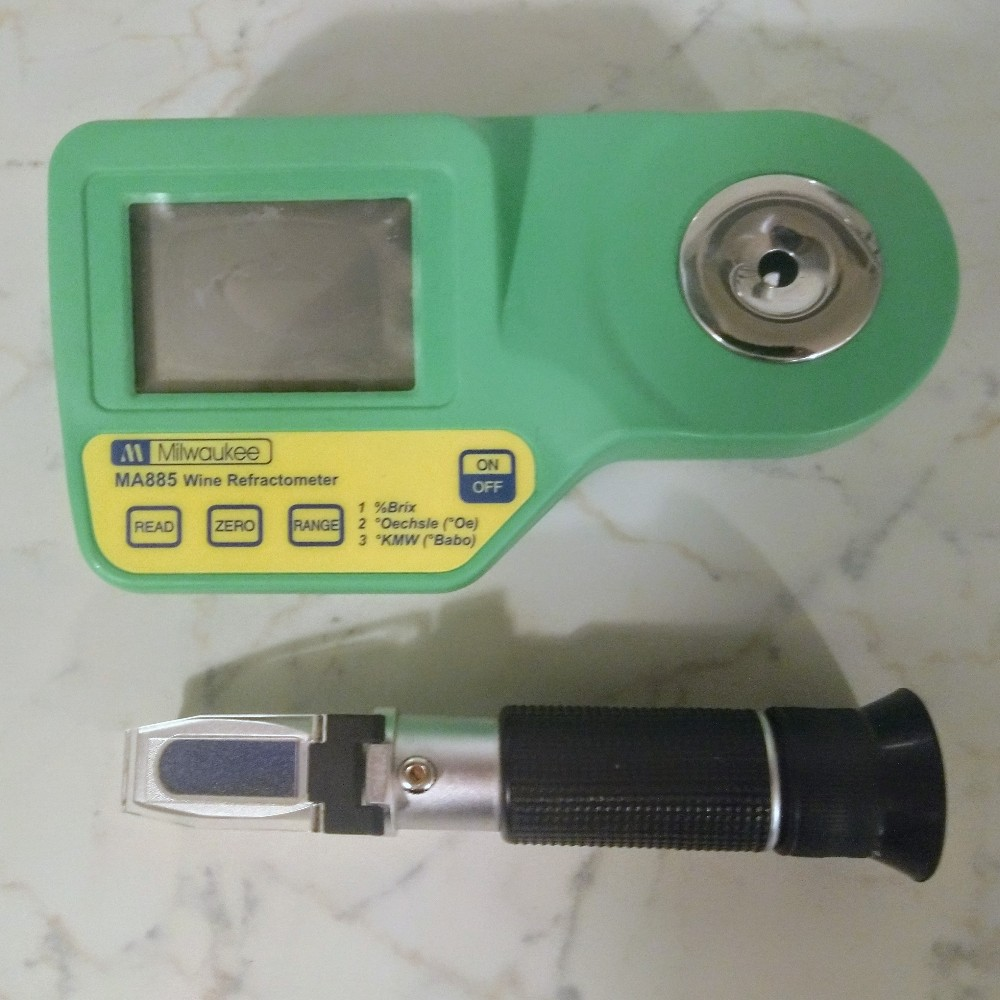
\includegraphics[width=4.8cm]{images/types.jpg}
%\caption{Typische Refraktometer im Heimbraubereich (Ascher, 2021)}
%\label{fig:refactotype}
%\end{figure}

\begin{table}[h]
\centering
\begin{tabular}{lrr}
\toprule
Parameter &  Handrefraktometer &  Milwaukee MA885 \\
\midrule
Preis [€] & 40 & 185 \\
Messbereich [°Bx] & 0--32 & 0--50 \\
Auflösung [°Bx] & 0,2 & 0,1 \\
Genauigkeit [°Bx] & 0,2 & 0,1 \\
ATC [°C] & 10--30 & 10--40 \\
Maßeinheiten & °Bx, SG & °Bx, °Oe, °KWM \\
Kalibrierschein & nein & ja \\
\bottomrule
\end{tabular}
\caption{Spezifikation typischer Refraktometer im Heimbraubereich  (Ascher, 2021)}
\label{table:refactospec}
\end{table}

\printbibliography[title=Quellen]

\end{document}